\documentclass[11pt]{article}

\usepackage{amsmath, amssymb}
\usepackage{geometry}
\usepackage{graphicx}
\graphicspath{{../figures/}{../figures/panels/}}
\usepackage{hyperref}
\usepackage{xcolor}
\usepackage{booktabs}
\usepackage{enumitem}

\geometry{margin=1.2in}

\hypersetup{
    colorlinks=true,
    linkcolor=blue!60!black,
    citecolor=blue!60!black,
    urlcolor=blue!60!black
}

% Match the figure typography: Computer Modern Sans Serif throughout.
\renewcommand{\familydefault}{\sfdefault}
\usepackage[T1]{fontenc}

% Notation shortcuts.
\newcommand{\Nzero}{N_0}
\newcommand{\bEdge}{b_e}
\newcommand{\dEdge}{d_e}
\newcommand{\bCore}{b_c}
\newcommand{\dCore}{d_c}
\newcommand{\bR}{b_R}
\newcommand{\dR}{d_R}
\newcommand{\sR}{s_R}

\title{Spatial rescue in biofilms:\\
a double-edged sword}
\author{}
\date{\today}

\begin{document}
\maketitle

\begin{abstract}
\noindent A biofilm under antibiotic treatment has a clear spatial
asymmetry: cells on the surface are exposed to the drug, while cells
in the deeper interior are shielded from it. We ask whether that
shielded interior makes the population more likely to evolve
resistance and survive (a process known as \emph{evolutionary rescue}). By comparing a spatially structured biofilm model
against a well-mixed population of the same initial size, and
sweeping the antibiotic dose along with the metabolic activity of
the interior, we find that the biofilm is a \emph{double-edged
sword}. When the interior is metabolically active, the biofilm
rescues less often than the well-mixed reference at low dose, but
more often at high dose. When the interior is dormant, the biofilm
has no rescue advantage at any dose and is uniformly less likely to evolve resistance than the well-mixed reference population.
\end{abstract}

% ---------------------------------------------------------------------------
\section{The question}
% ---------------------------------------------------------------------------

The current antibiotic resistance crisis is a major public health threat, and biofilms are a key part of the problem. Biofilms are dense, surface-attached communities of bacteria that are common in nature and in infections. They are notoriously hard to kill with antibiotics, and they are thought to be responsible for a large fraction of chronic infections. Understanding how biofilms evolve resistance under antibiotic treatment is therefore an important question. Furthermore, treating infections with behavior-modifying interventions, such that a compound may induce increased biofilm formation, or increased dispersal (towards a well-mixed population), is an active area of research. The intuition is that while antibiotics induce high killing selective pressure, behavior-modifying interventions may not kill bacteria, but could reduce the population's ability to evolve antibiotic resistance by disrupting the spatial structure of the biofilm. To predict the evolutionary consequences of such interventions, we need to understand how the spatial structure of a biofilm affects the population's ability to evolve resistance in the first place, and whether applying such a treatment is likely to help or hurt the population's chances of survival when applied in conjunction with antibiotics. 

Moreover, to treat bacterial infections effectively, we need to understand the evolutionary dynamics of resistance not in a simple well-mixed culture, but in the complex spatial structure of a biofilm. The spatial structure creates a natural asymmetry: cells on the surface are exposed to the drug, while cells in the deeper interior are shielded from it. This shielded interior is a spatial refuge that could potentially allow the population to survive longer under treatment, and therefore give it more time to evolve resistance. But does it actually help the population survive in the long run? Thus, we set out to answer whether the structure of a biofilm actually helps the population survive in the long run, by allowing \emph{evolutionary rescue}: the outcome in which a declining population avoids extinction because a resistant mutant arises and takes over in time.

The naive intuition is that the refuge provided by a biofilm should help a population evolve drug resistance. A shielded interior keeps the population around for longer timescales, so more mutations have a chance to arise. But more mutations is not the same thing as more rescue. For a mutation to matter, it has to reach the drug-exposed surface and grow there. Mutations stuck in the shielded interior do nothing on their own, because the interior carries no selection pressure to give a resistant cell its advantage. Whether the biofilm is a net help or a net hindrance to a population aiming to survive through evolving antibiotic resistance therefore depends on how effectively interior mutations make it to the surface, and on whether the spatial structure carries hidden costs that offset the supply benefit. That is what we set out to measure.



% ---------------------------------------------------------------------------
\section{The model}
\label{sec:model}
% ---------------------------------------------------------------------------

The biofilm is a one-dimensional chain of cells. The outermost $l$ cells of the chain form the \textbf{edge}, where the antibiotic is
present. Everything deeper forms the \textbf{core}, where the
antibiotic does not reach. Each cell is either wild-type (WT) or
resistant (R). Resistance is irreversible: an R cell can only
produce R daughters.

\subsection{Birth and death rates}
Each cell has a birth rate and a death rate that depend on its
compartment and its genotype.
\begin{itemize}
    \item \textbf{Edge, WT}: Birth rate $\bEdge = 1$, which sets the
    time unit. Death rate $\dEdge$ is the antibiotic dose. We sweep
    over values $\dEdge > \bEdge$, so WT cells in the edge are
    always net-dying under treatment.
    \item \textbf{Edge, R}: Resistant cells in the edge have birth
    rate $\bR = 1$ and death rate $\dR = 0.6$. Their net growth rate
    $\sR = \bR - \dR = 0.4$ is positive, so once an R lineage
    establishes, it grows.
    \item \textbf{Core, WT and R}: Cells in the core have balanced
    birth and death rates, $\bCore = \dCore$, so the core has no net
    growth on its own. WT and R cells are treated identically in the
    core, since the shielded interior carries no selection pressure.
    The default core activity is $\bCore = 0.2$, a slow but nonzero
    rate. A fully dormant interior corresponds to $\bCore = 0$.
\end{itemize}

\subsection{Two phases of decline}
The core and edge are mechanically coupled by a simple bookkeeping
rule: as long as the core still has cells in it, the edge always
contains exactly $l$ cells. Whenever an edge cell divides, the
population grows by one and the innermost edge cell is reclassified
as a core cell, to maintain the fixed edge length $l$. Whenever an edge cell dies, the population shrinks
by one and the outermost core cell is reclassified as an edge cell.
This rule produces two regimes of decline.
\begin{enumerate}
    \item \textbf{Buffered decline} (phase of simulation where core is still present). When there there still cells left in the core (ie., $n(t) > l$), each death in the edge is immediately replaced by a cell drawn from the core, so the edge stays at $l$ cells. Only the $l$ edge cells
    contribute to net loss, and the total population falls linearly.
    \item \textbf{Final collapse} (phase of simulation where core is gone). When the core is exhausted (ie., $N(t) \leq l$), the edge is the entire remaining population. There is no reservoir from the core left to draw on, and the remaining cells decay exponentially, just as a well-mixed population would.
\end{enumerate}
The buffered decline lasts a long time at low dose, when slow edge
turnover gradually drains the core. It is brief at high dose, when
fast edge turnover quickly burns through the core.

\subsection{Mutations and rescue.}
Each birth event has a small probability $\mu$ of producing a
resistant daughter instead of a wild-type one. Mutations can arise
in either compartment. Because the core's birth rate is lower than
the edge's, core cells generate mutations more slowly per unit time
than edge cells do. A run counts as rescued once at least
$r_{\text{thr}} = 10$ resistant cells are present in the edge at
the same time, a count large enough to virtually guarantee takeover.

\subsection{The reference: a well-mixed population (Wilson et al. 2017).}
To say whether the biofilm helps or hurts, we compare against a
well-mixed population of the same initial size $\Nzero$, using Benjamin Wilson's evolutionary rescue framework (Wilson et al. 2017), excluding the soft sweep detection that was specific to Wilson's model. The
well-mixed population is the one-compartment analog of the chain model, and uses only the edge rates: every cell is drug-exposed, with no shielded interior. This is the standard setting for evolutionary rescue.



\section{Parameters and simulation conditions}
\label{sec:params}


Time is measured in edge generations ($\bEdge = 1$). We use a Gillespie
stochastic simulation, with one event sampled at a time according to
current rates.

\begin{table}[htbp]
\centering
\small
\begin{tabular}{lll}
\toprule
Parameter & Value & Meaning \\
\midrule
$\Nzero$         & $1000$        & Initial population size \\
$l$              & $100$         & Edge width (cells exposed to drug) \\
$\bEdge$         & $1.0$         & WT birth rate in edge (sets time unit) \\
$\dEdge$         & dose (swept)  & WT death rate in edge; super-MIC is $\dEdge > 1$ \\
$\bR$            & $1.0$         & R birth rate in edge \\
$\dR$            & $0.6$         & R death rate in edge ($\sR = 0.4$) \\
$\bCore = \dCore$ & $0.2$ (swept) & Core birth/death rate (active by default; $0$ = dormant) \\
$\mu$            & $10^{-4}$     & Mutation probability per birth \\
$r_{\text{thr}}$ & $10$          & Resistant edge cells required to declare rescue \\
\bottomrule
\end{tabular}
\caption{Default model parameters. The two swept variables are dose
($\dEdge$), core activity ($\bCore$), and edge length ($l$).}
\end{table}

We sweep dose over $\dEdge \in \{1.05,\,1.1,\,1.2,\,1.4,\,1.6,\,1.9,\,
2.3,\,2.8\}$, core activity over $\bCore \in \{0,\,0.05,\,0.1,\,0.2,\,0.4,\,0.8\}$, and edge length $l \in \{0, 25, 50, 100, 200, 400\}$ with $5{,}000$ independent runs at every parameter combination. The well-mixed
reference is run at the same set of doses, also $5{,}000$ replicates per
dose. Every run terminates naturally on either rescue ($r_{\text{edge}} \geq r_{\text{thr}}$) or extinction ($N = 0$); no
artificial time or generation cap is applied.



\section{The double-edged sword}
\label{sec:doubleedge}


To see whether the biofilm helps or hurts, we pick two doses at opposite
ends of the swept range---a low dose just above the minimum inhibitory
concentration ($\dEdge = 1.05$) and a high dose well above it
($\dEdge = 2.8$)---and compare the biofilm's rescue probability against
the well-mixed population's at each. We run that comparison twice: once
with a dormant core ($\bCore = 0$), and once with a highly active core
($\bCore = 0.8$). The four resulting comparisons are shown together in
Figure~\ref{fig:doubleedge}.

\begin{figure}[htbp]
\centering
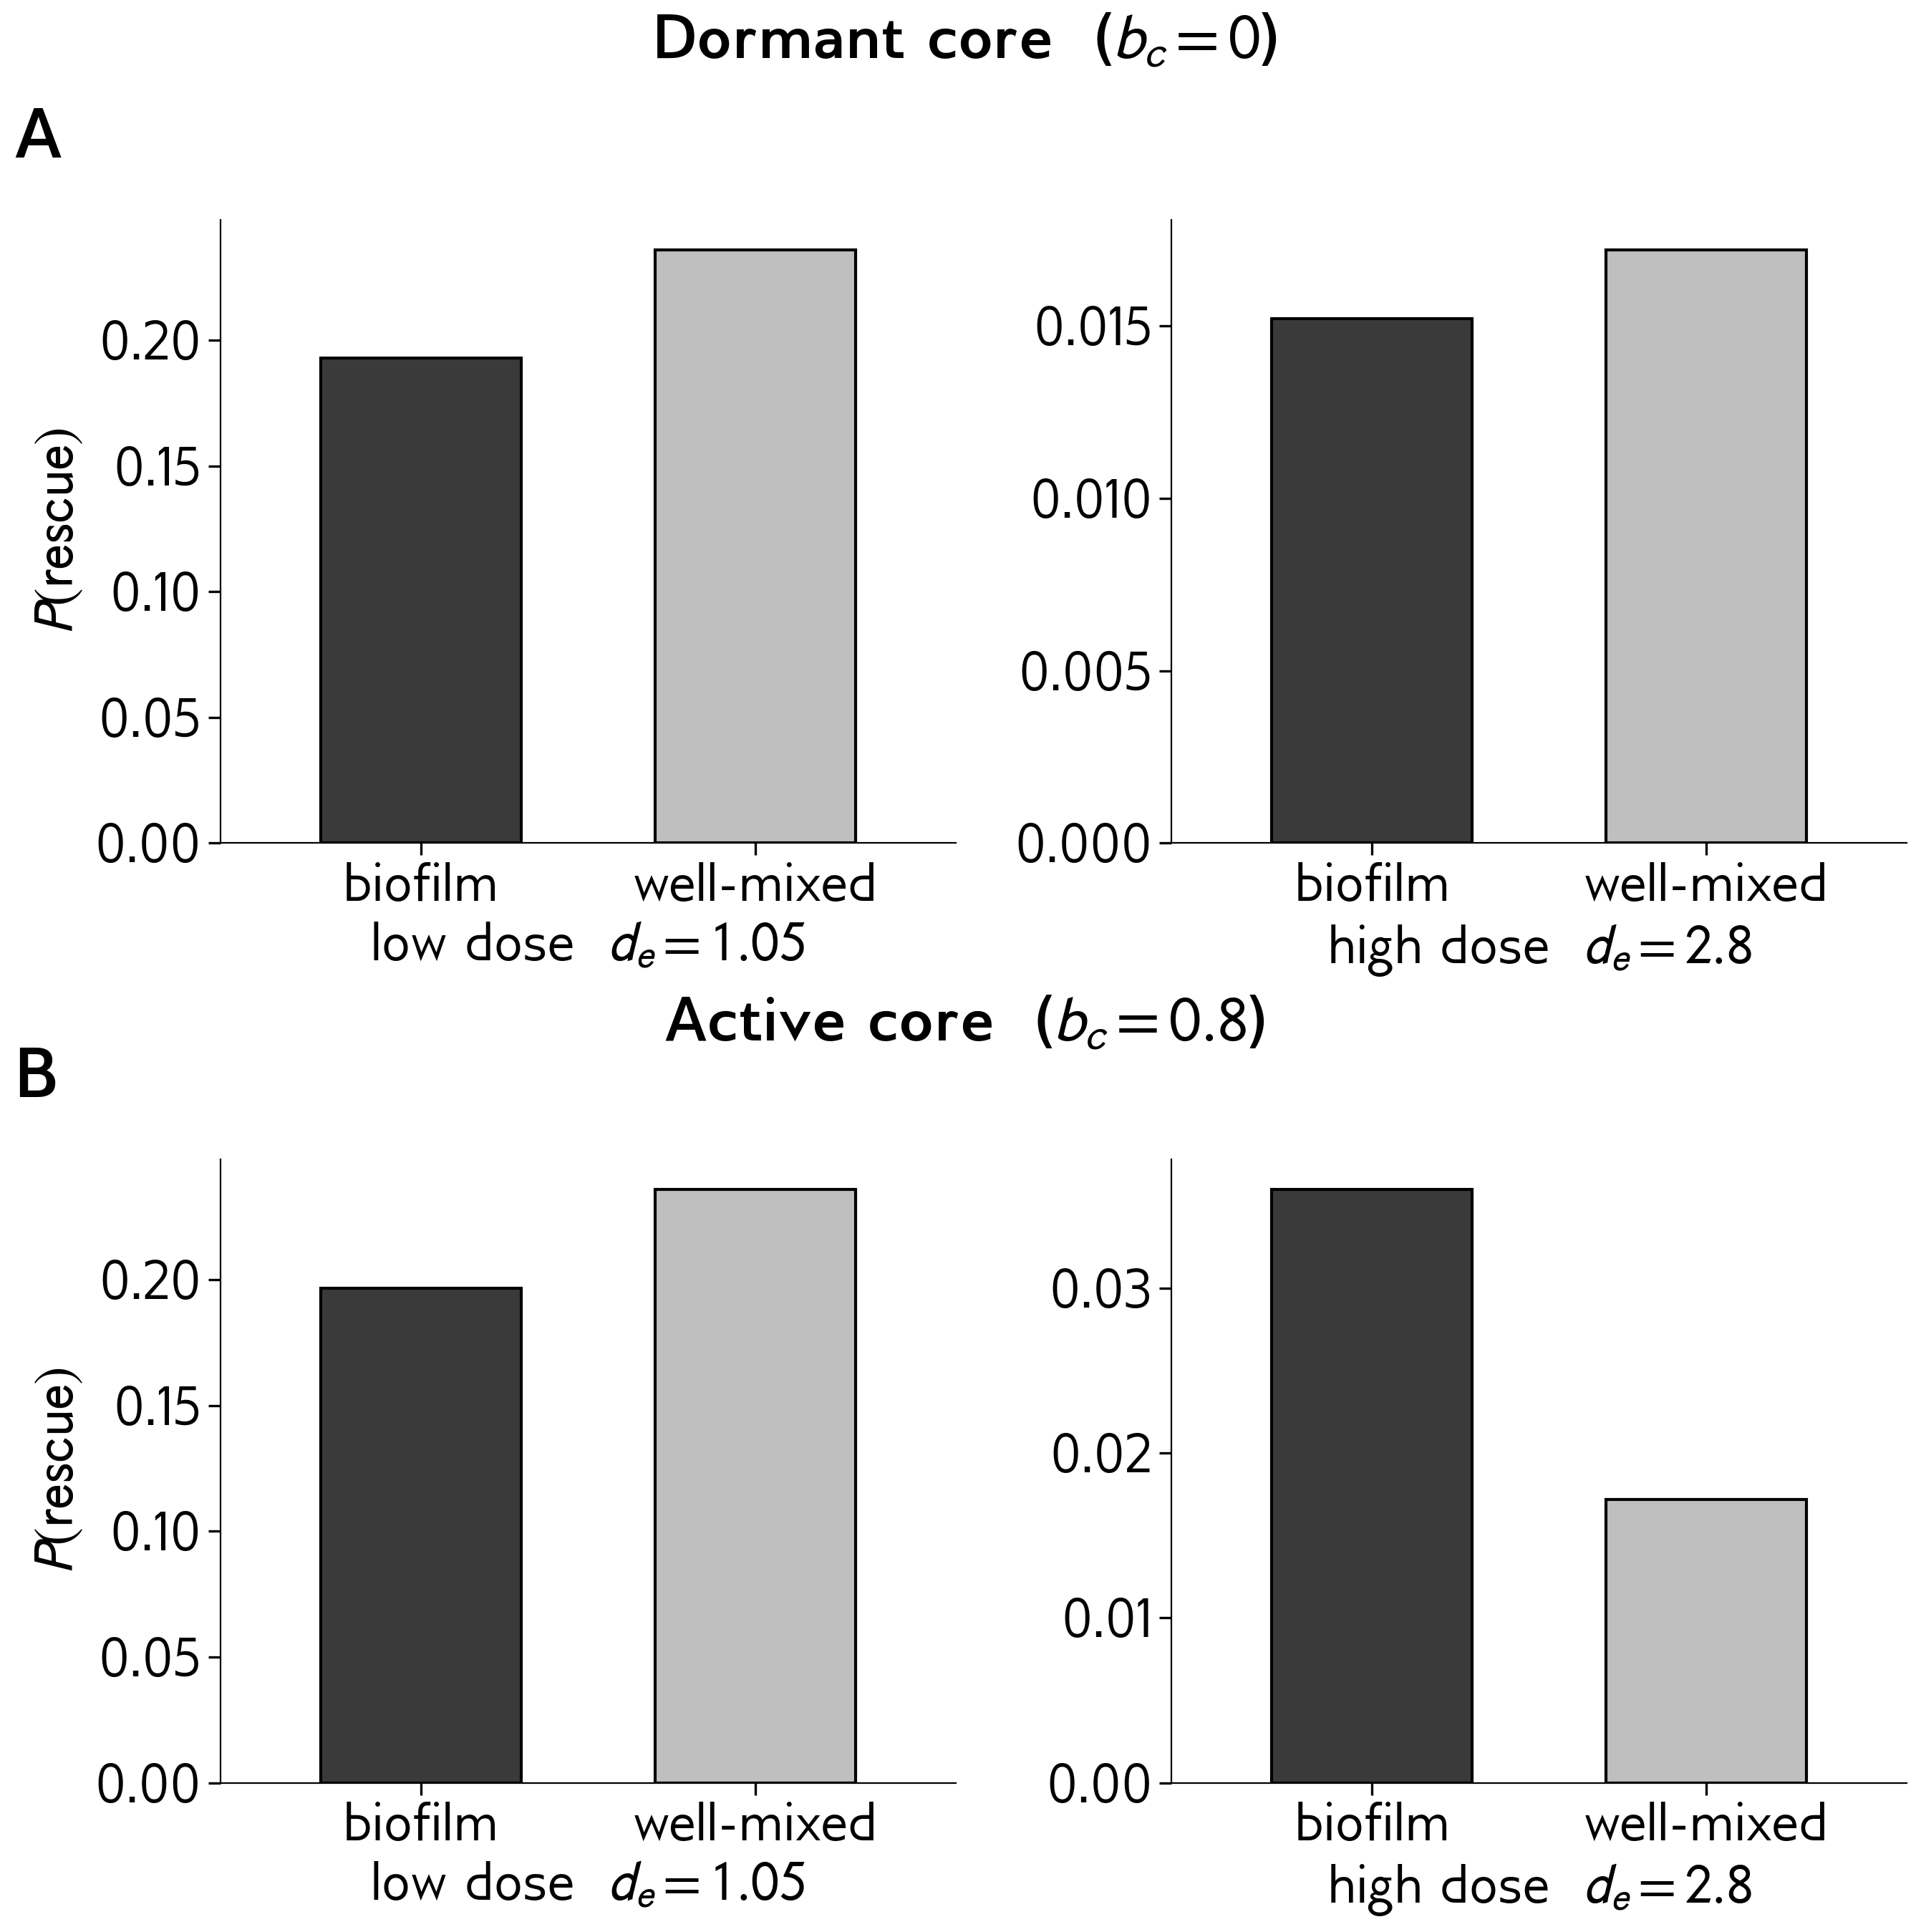
\includegraphics[width=0.75\textwidth]{double_edge_rescue.png}
\caption{Rescue probability for the biofilm (dark) versus the well-mixed
reference (light), at low dose ($\dEdge = 1.05$, left columns) and high
dose ($\dEdge = 2.8$, right columns). \textbf{Panel A}: dormant core
($\bCore = 0$). \textbf{Panel B}: active core ($\bCore = 0.8$). Each
subplot uses its own y-axis scale. \emph{Parameters}: $N_0 = 1000$,
$l = 100$, $\mu = 10^{-4}$; each bar averages over 5{,}000 independent
simulation runs.}
\label{fig:doubleedge}
\end{figure}

\paragraph{Panel A: dormant core.}
When the interior cannot divide, the biofilm rescues less often than the
well-mixed population at both doses. The well-mixed bar is taller in
each subplot. The shielded interior does not buy any benefit when
nothing is happening inside it---the spatial structure is purely a
liability.

\paragraph{Panel B: active core.}
When the interior is dividing at a steady rate, the picture splits in
two. At low dose, the biofilm still loses---just as in Panel A. But at
high dose the bars flip: the biofilm rescues roughly \emph{twice} as
often as the well-mixed reference. The same spatial structure that
hurts at low dose now helps at high dose. This is the double-edged
sword.

\paragraph{What this means together.}
The biofilm only wins under one specific combination: high dose plus an
active core. Neither piece is enough on its own:
\begin{itemize}
    \item A dormant core never helps, no matter the dose.
    \item An active core only helps at high dose; at low dose it still
    loses.
\end{itemize}
The two conditions have to coincide for the spatial structure to pay
off.

This raises two follow-up questions. Why does the biofilm consistently
lose at low dose, regardless of how active the core is? And what does
an active core contribute at high dose that it does not contribute at
low dose? The rest of the writeup works through these mechanisms.



\section{Rescue probability across dose}
\label{sec:dosecurves}


The bar plot in Figure~\ref{fig:doubleedge} sampled two specific
doses at opposite ends of the swept range. To see whether the flip
between them is a smooth crossover or just a jump between two
unrelated regimes, we plot rescue probability across the full
range of doses we swept (Figure~\ref{fig:dosecurves}).

\begin{figure}[htbp]
\centering
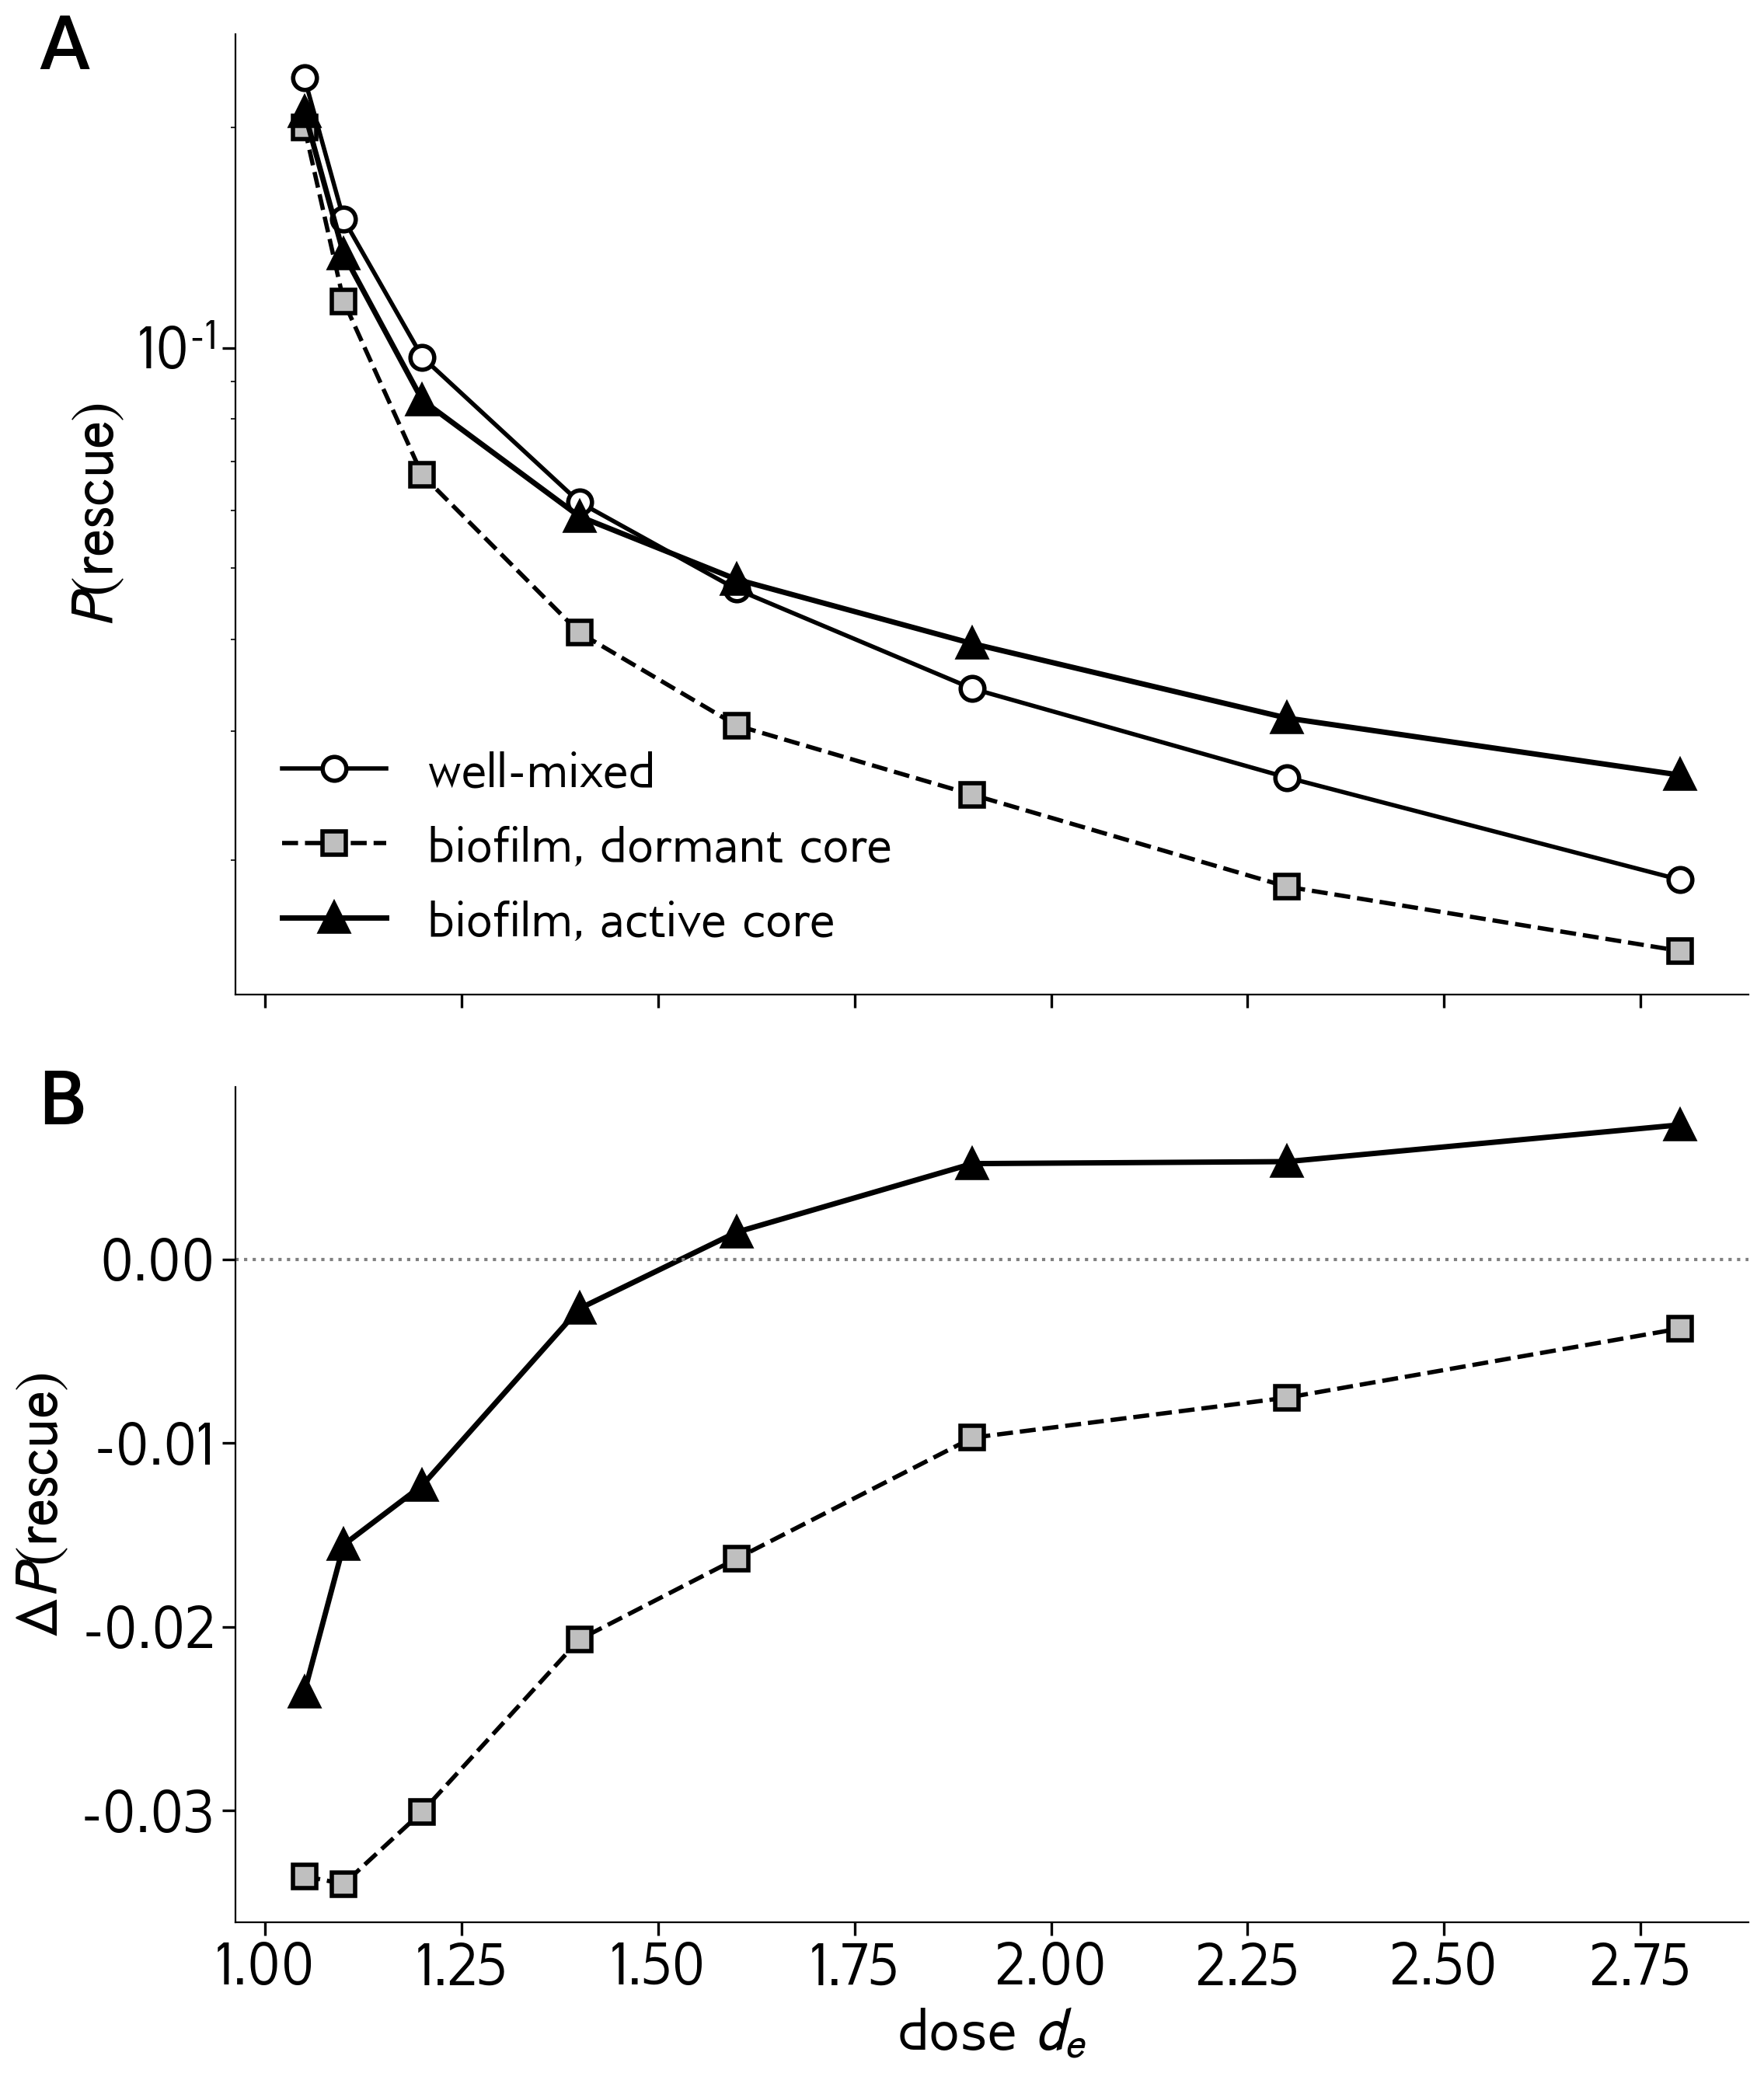
\includegraphics[width=0.85\textwidth]{dose_curves_rescue.png}
\caption{Rescue probability across dose, for the three conditions in
Figure~\ref{fig:doubleedge}. The biofilm with a dormant core (dashed)
stays below the well-mixed reference at every dose; no crossing
exists. The biofilm with an active core (solid triangles) crosses
above the well-mixed line around $\dEdge \approx 1.4$ and stays above
it at higher doses. \emph{Parameters}: $N_0 = 1000$, $l = 100$,
$\mu = 10^{-4}$; each point averages over 5{,}000 runs.}
\label{fig:dosecurves}
\end{figure}

The active-core biofilm crosses the well-mixed reference smoothly,
at $\dEdge \approx 1.4$. Below that dose the biofilm loses; above
it, the biofilm wins. The flip seen in the bar plot is one
continuous crossover, not two separate effects.

The dormant-core biofilm does not cross at all. Its curve runs
strictly below the well-mixed reference at every dose. The
``double-edged sword'' is therefore specifically a property of
biofilms with metabolically active cores; a biofilm with a dormant
interior is simply a worse rescue substrate than well-mixed at
every dose.

\paragraph{Does the crossover depend on biofilm geometry?}
The curves above were all computed at one edge width, $l = 100$
cells out of $N_0 = 1000$. Real biofilms come in different
thicknesses, and real antibiotics penetrate to different depths,
so $l$ is not a fixed quantity in the natural setting we are trying
to model. Before trying to explain the crossover, it is worth
checking whether it survives changes in $l$. Figure~\ref{fig:sensl}
sweeps $l$ over a sixteenfold range while holding everything else
fixed.

\begin{figure}[htbp]
\centering
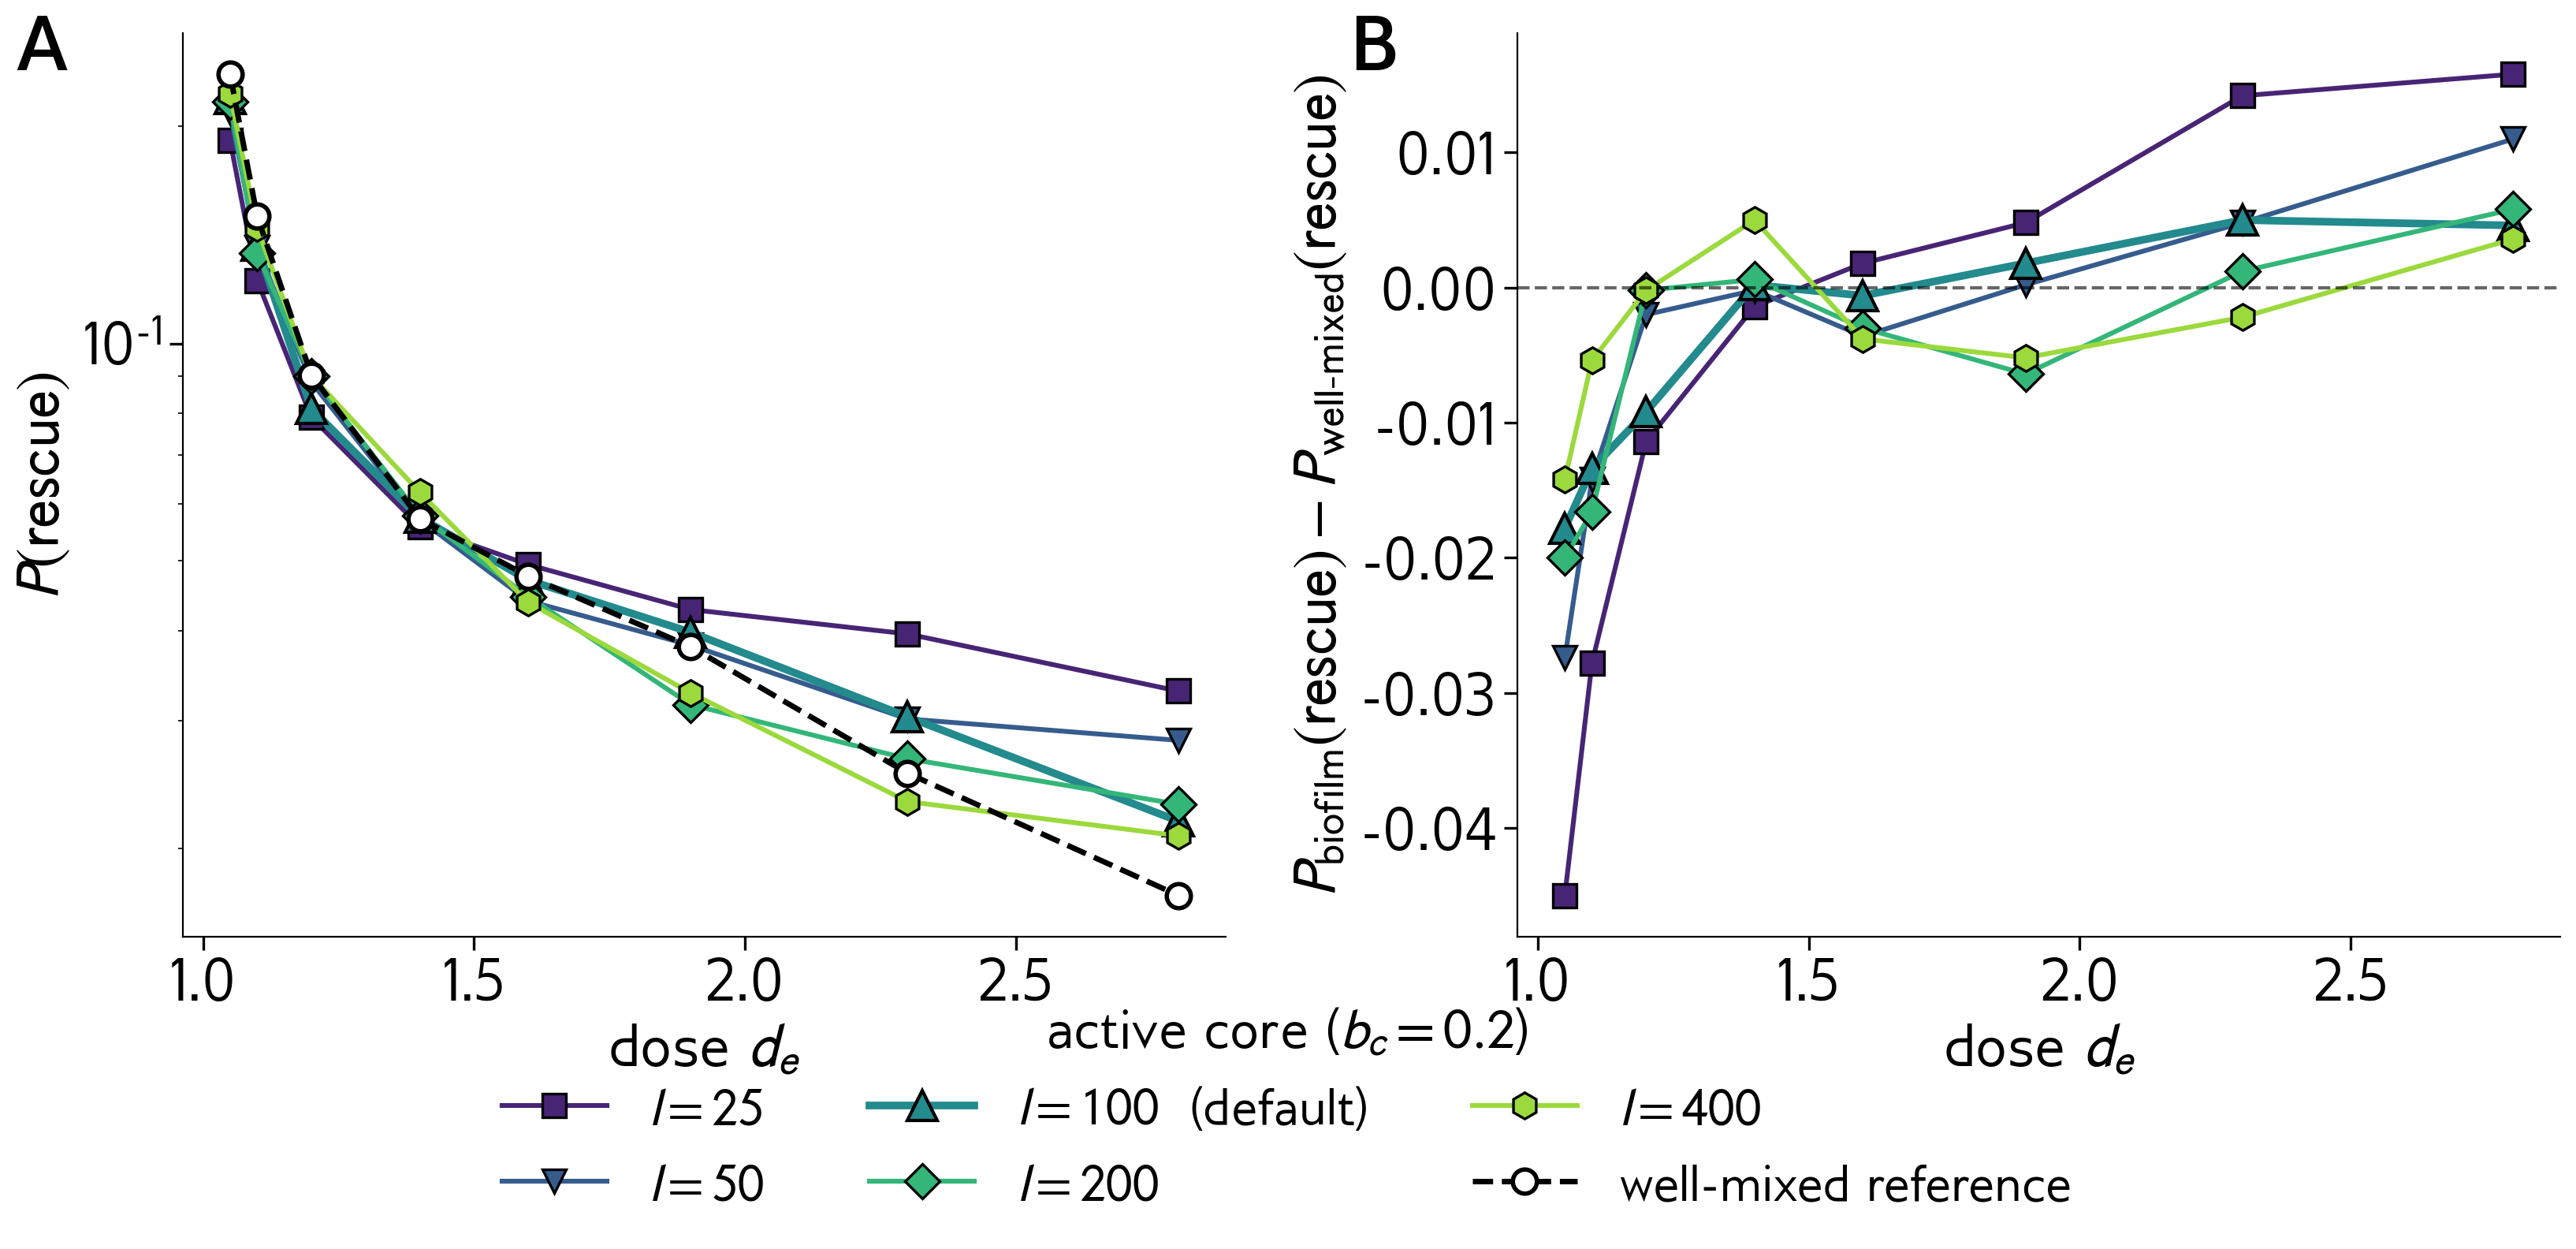
\includegraphics[width=0.97\textwidth]{sensL_curves.png}
\caption{Two-panel view of the $l$ sweep.
\textbf{Panel A}: rescue probability across dose at every edge width
in our sweep ($l \in \{25, 50, 100, 200, 400\}$) alongside the
well-mixed reference. \textbf{Panel B}: the biofilm-minus-well-mixed
difference $P_{\mathrm{BF}}(\text{rescue}) - P_{\mathrm{WM}}(\text{rescue})$.
The crossover is the zero crossing in Panel B; the high-dose advantage
is the height of each curve above zero. All five biofilm curves
converge to the well-mixed value at low dose and diverge at high dose,
with smaller $l$ giving a larger high-dose biofilm advantage. The
qualitative double-edge pattern is a structural feature of the model,
not an artifact of one particular $l$. \emph{Parameters}: $N_0 = 1000$,
$\bCore = 0.2$ (the sensitivity sweep's active-core value),
$\mu = 10^{-4}$; each point averages over 5{,}000 runs.}
\label{fig:sensl}
\end{figure}

The crossover survives. At every $l$ in our sweep---a thin edge
over a thick core ($l = 25$), a thick edge over a thin core
($l = 400$), and everything in between---the biofilm starts below
the well-mixed reference at low dose and ends up above it at high
dose. The crossover is structural, not a quirk of one specific
geometry.

What does shift with $l$ is the \emph{location} of the crossover.
Smaller $l$ (a thinner edge sitting on top of a thicker core)
pushes the crossover to a lower dose, and gives the biofilm a
larger advantage at high dose. Larger $l$ pushes the crossover
later. Figure~\ref{fig:xover} summarizes this dependence by
extracting one crossover dose per $l$.

\begin{figure}[htbp]
\centering
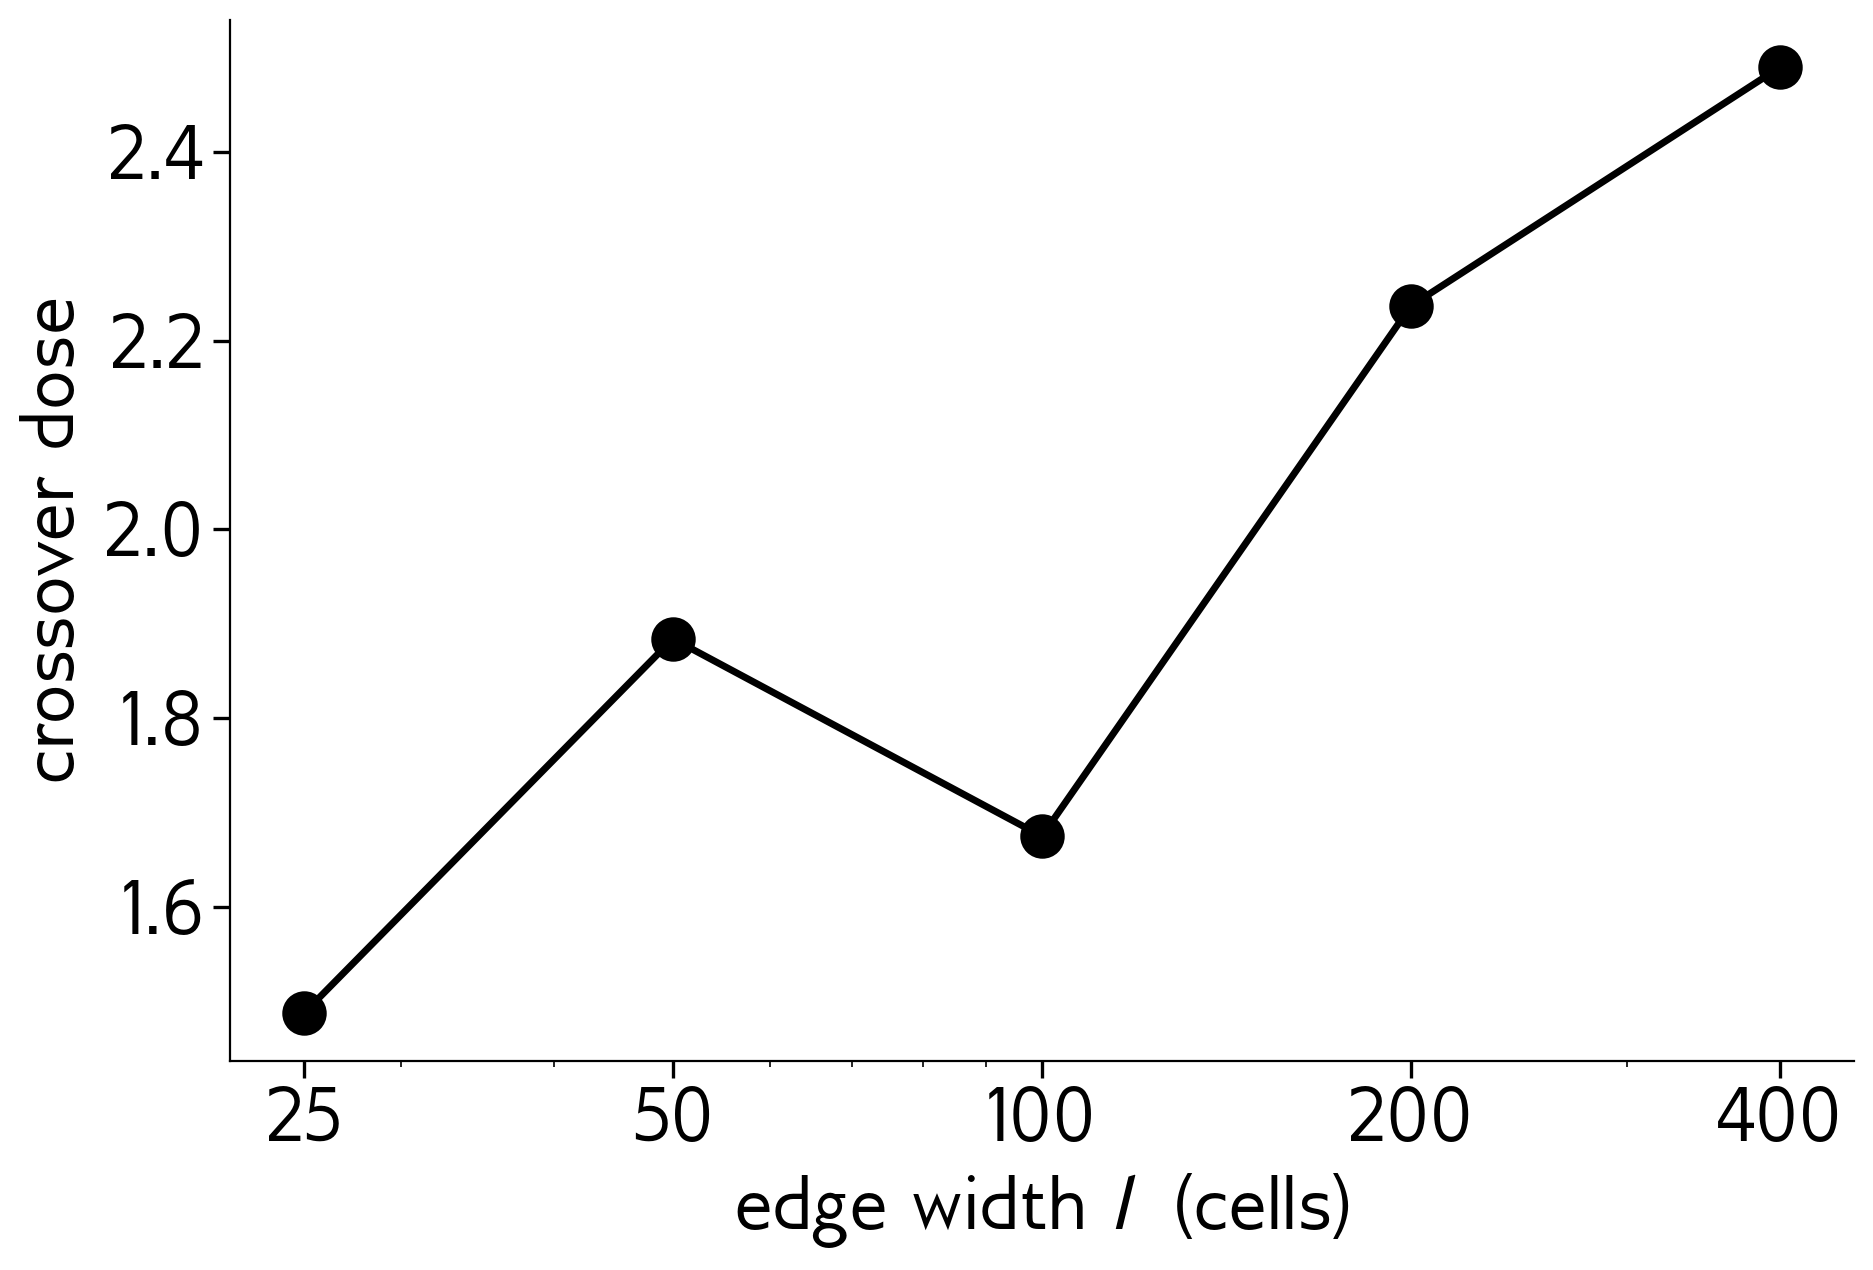
\includegraphics[width=0.65\textwidth]{crossover_vs_l.png}
\caption{Crossover dose (the dose above which the biofilm rescues
more often than the well-mixed reference at \emph{every} higher
dose) as a function of edge width $l$. For each $l$ in
Figure~\ref{fig:sensl}, we identify the largest sampled dose at
which the biofilm is still at or below well-mixed, and linearly
interpolate $P_{\mathrm{BF}} - P_{\mathrm{WM}}$ between that dose
and the next-higher sampled dose (where the biofilm has gone above)
to find the zero. The overall trend is increasing---thinner edges
give earlier crossovers---and the small bump at $l = 50$ is
consistent with sampling noise: the biofilm and well-mixed rescue
probabilities differ by $\lesssim 0.004$ in the crossover region,
near the resolution limit of 5{,}000 seeds. \emph{Parameters}: same
as Figure~\ref{fig:sensl}.}
\label{fig:xover}
\end{figure}

The crossover dose increases with $l$. A thinner edge and a
thicker core push the crossover earlier; a thicker edge and a
thinner core delay it.

\paragraph{Does the crossover depend on how active the core is?}
Section~\ref{sec:doubleedge} showed that a fully dormant core
($\bCore = 0$) wipes out the biofilm's high-dose advantage entirely:
the biofilm rescues less often than well-mixed at both ends of the
dose range. An active core ($\bCore = 0.8$) restored the advantage.
We now sweep $\bCore$ across the intermediate range to find out how
active the core actually has to be for the crossover to appear, and
how the crossover dose moves with $\bCore$. Figure~\ref{fig:senscore}
shows the dose curves and their well-mixed difference for the full
$\bCore$ sweep.

\begin{figure}[htbp]
\centering
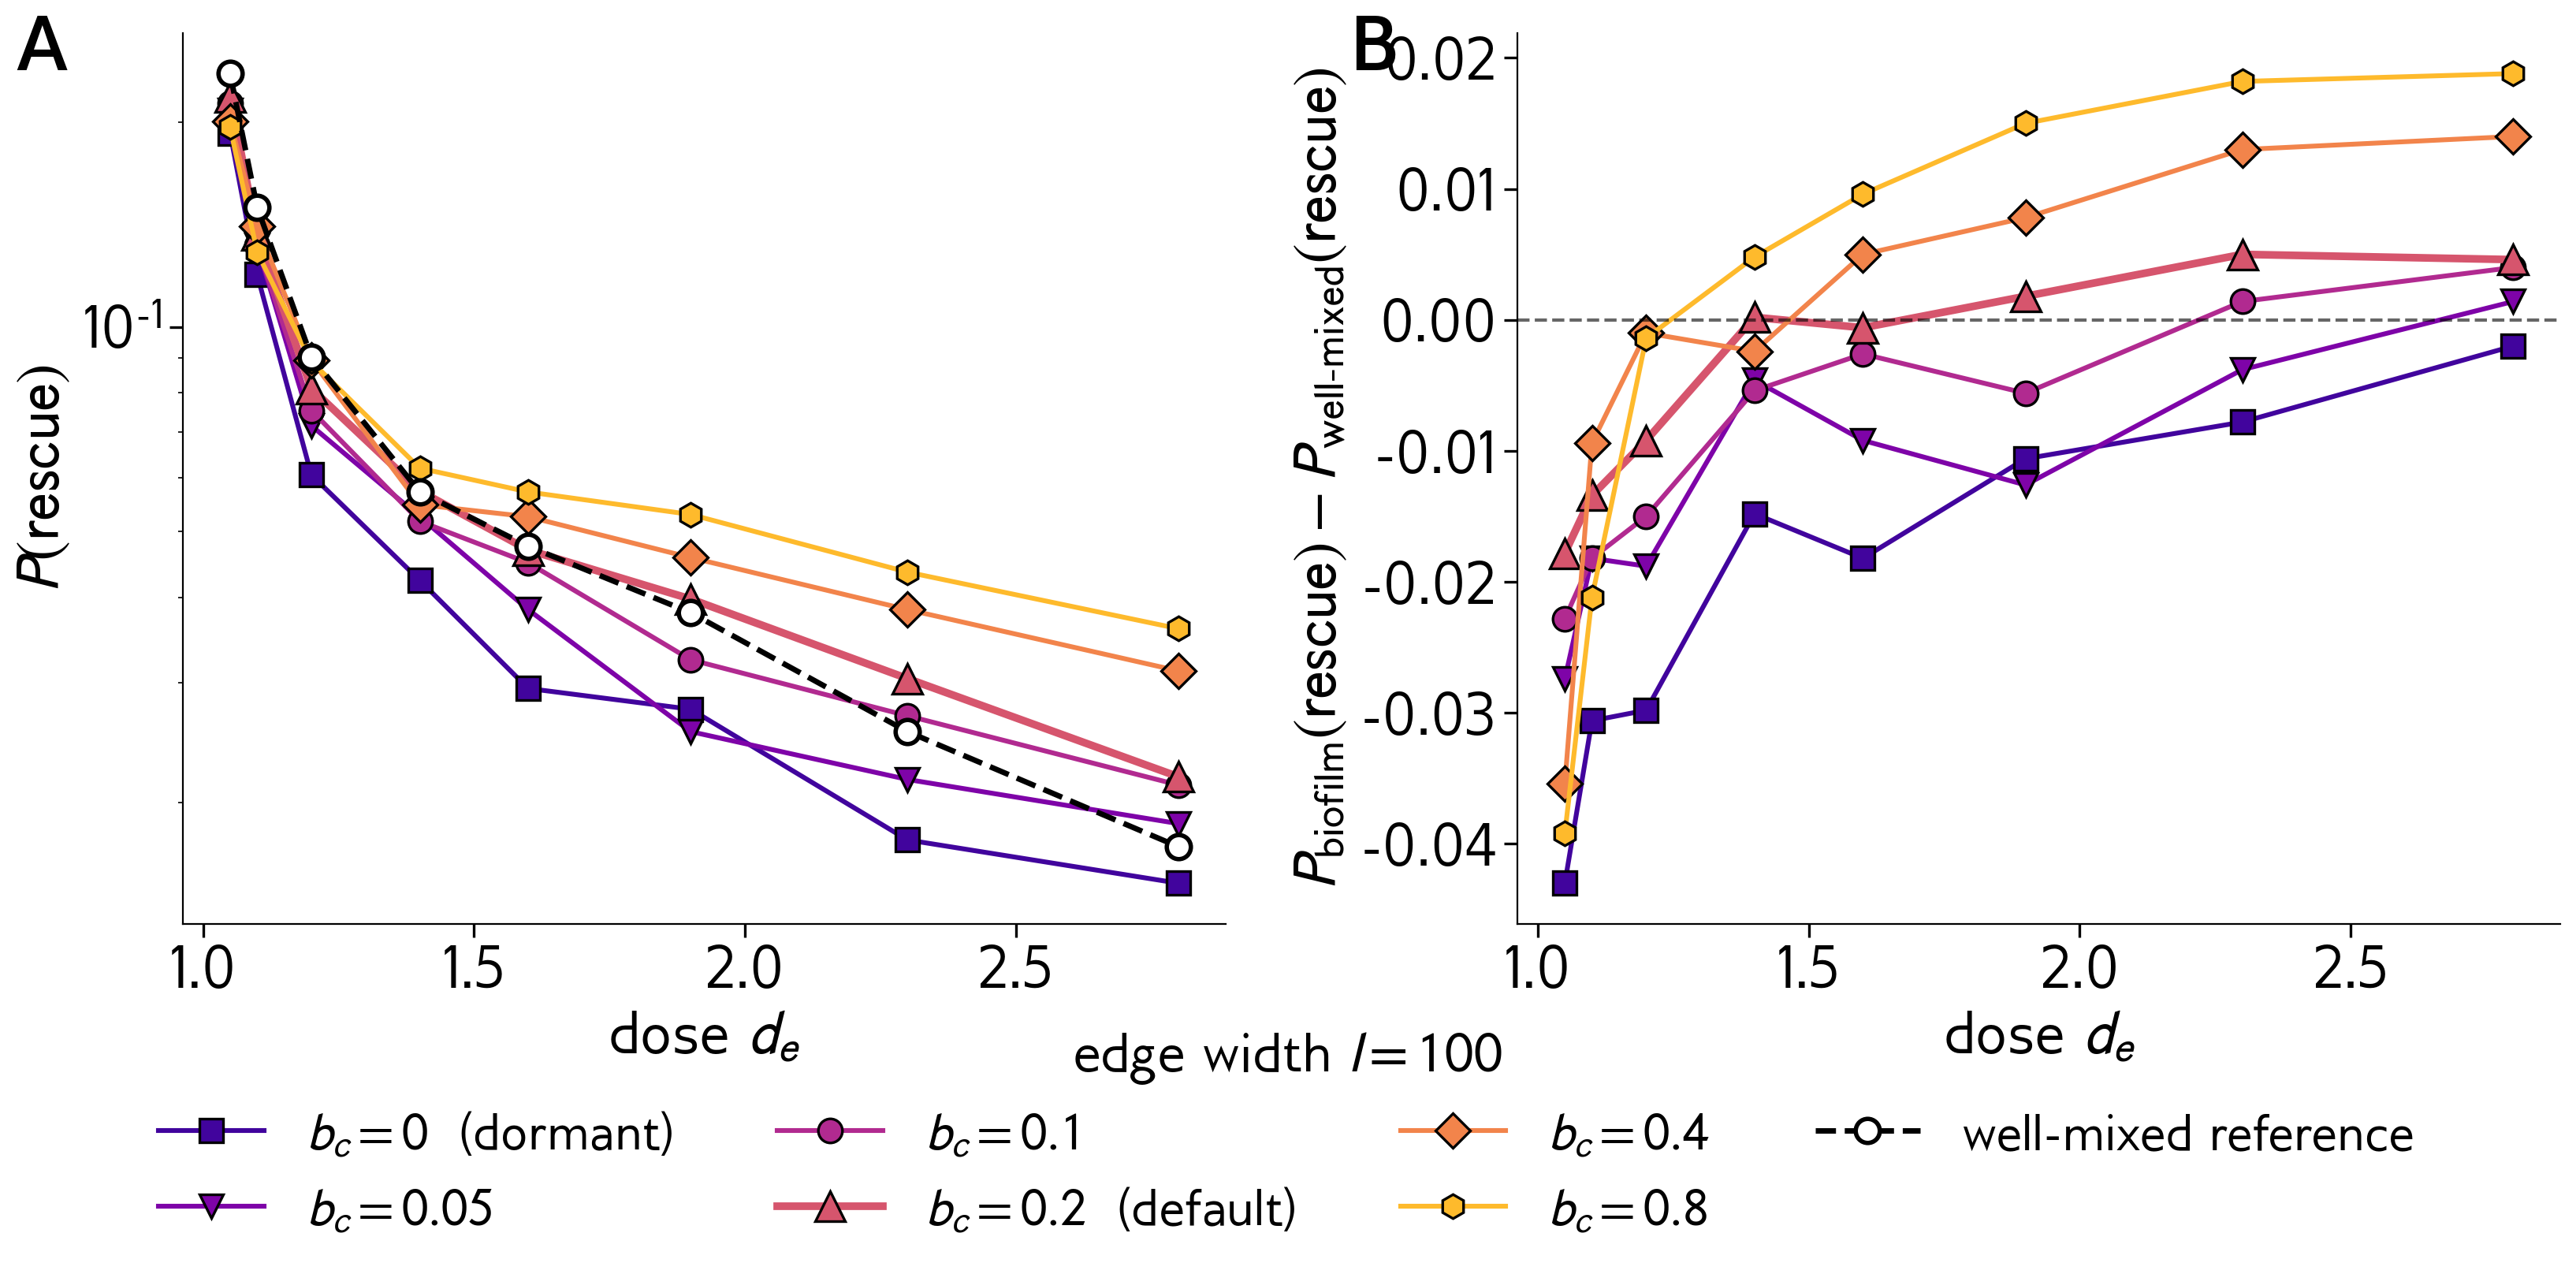
\includegraphics[width=0.97\textwidth]{sensCore_curves.png}
\caption{Two-panel view of the $\bCore$ sweep, at fixed $l = 100$.
\textbf{Panel A}: rescue probability across dose at every core
activity in our sweep
($\bCore \in \{0,\,0.05,\,0.1,\,0.2,\,0.4,\,0.8\}$) alongside the
well-mixed reference. \textbf{Panel B}: the biofilm-minus-well-mixed
difference. The dormant ($\bCore = 0$) curve sits strictly below zero
at every dose---no crossover exists. Every other curve crosses zero
somewhere in the swept range and sits above zero at high dose. The
high-dose advantage grows monotonically with $\bCore$.
\emph{Parameters}: $N_0 = 1000$, $l = 100$, $\mu = 10^{-4}$; each
point averages over 5{,}000 runs.}
\label{fig:senscore}
\end{figure}

The picture is clean: $\bCore = 0$ has no crossover, while every
positive $\bCore$ in the sweep does. Even a very slow core
($\bCore = 0.05$, one-twentieth of the edge birth rate) is enough
to produce a crossover, although it sits at a very high dose. As
$\bCore$ increases, the crossover moves to lower doses and the
high-dose advantage grows. Figure~\ref{fig:xover_bc} summarizes the
relationship by extracting one crossover dose per $\bCore$, using the
same strict definition as Figure~\ref{fig:xover}.

\begin{figure}[htbp]
\centering
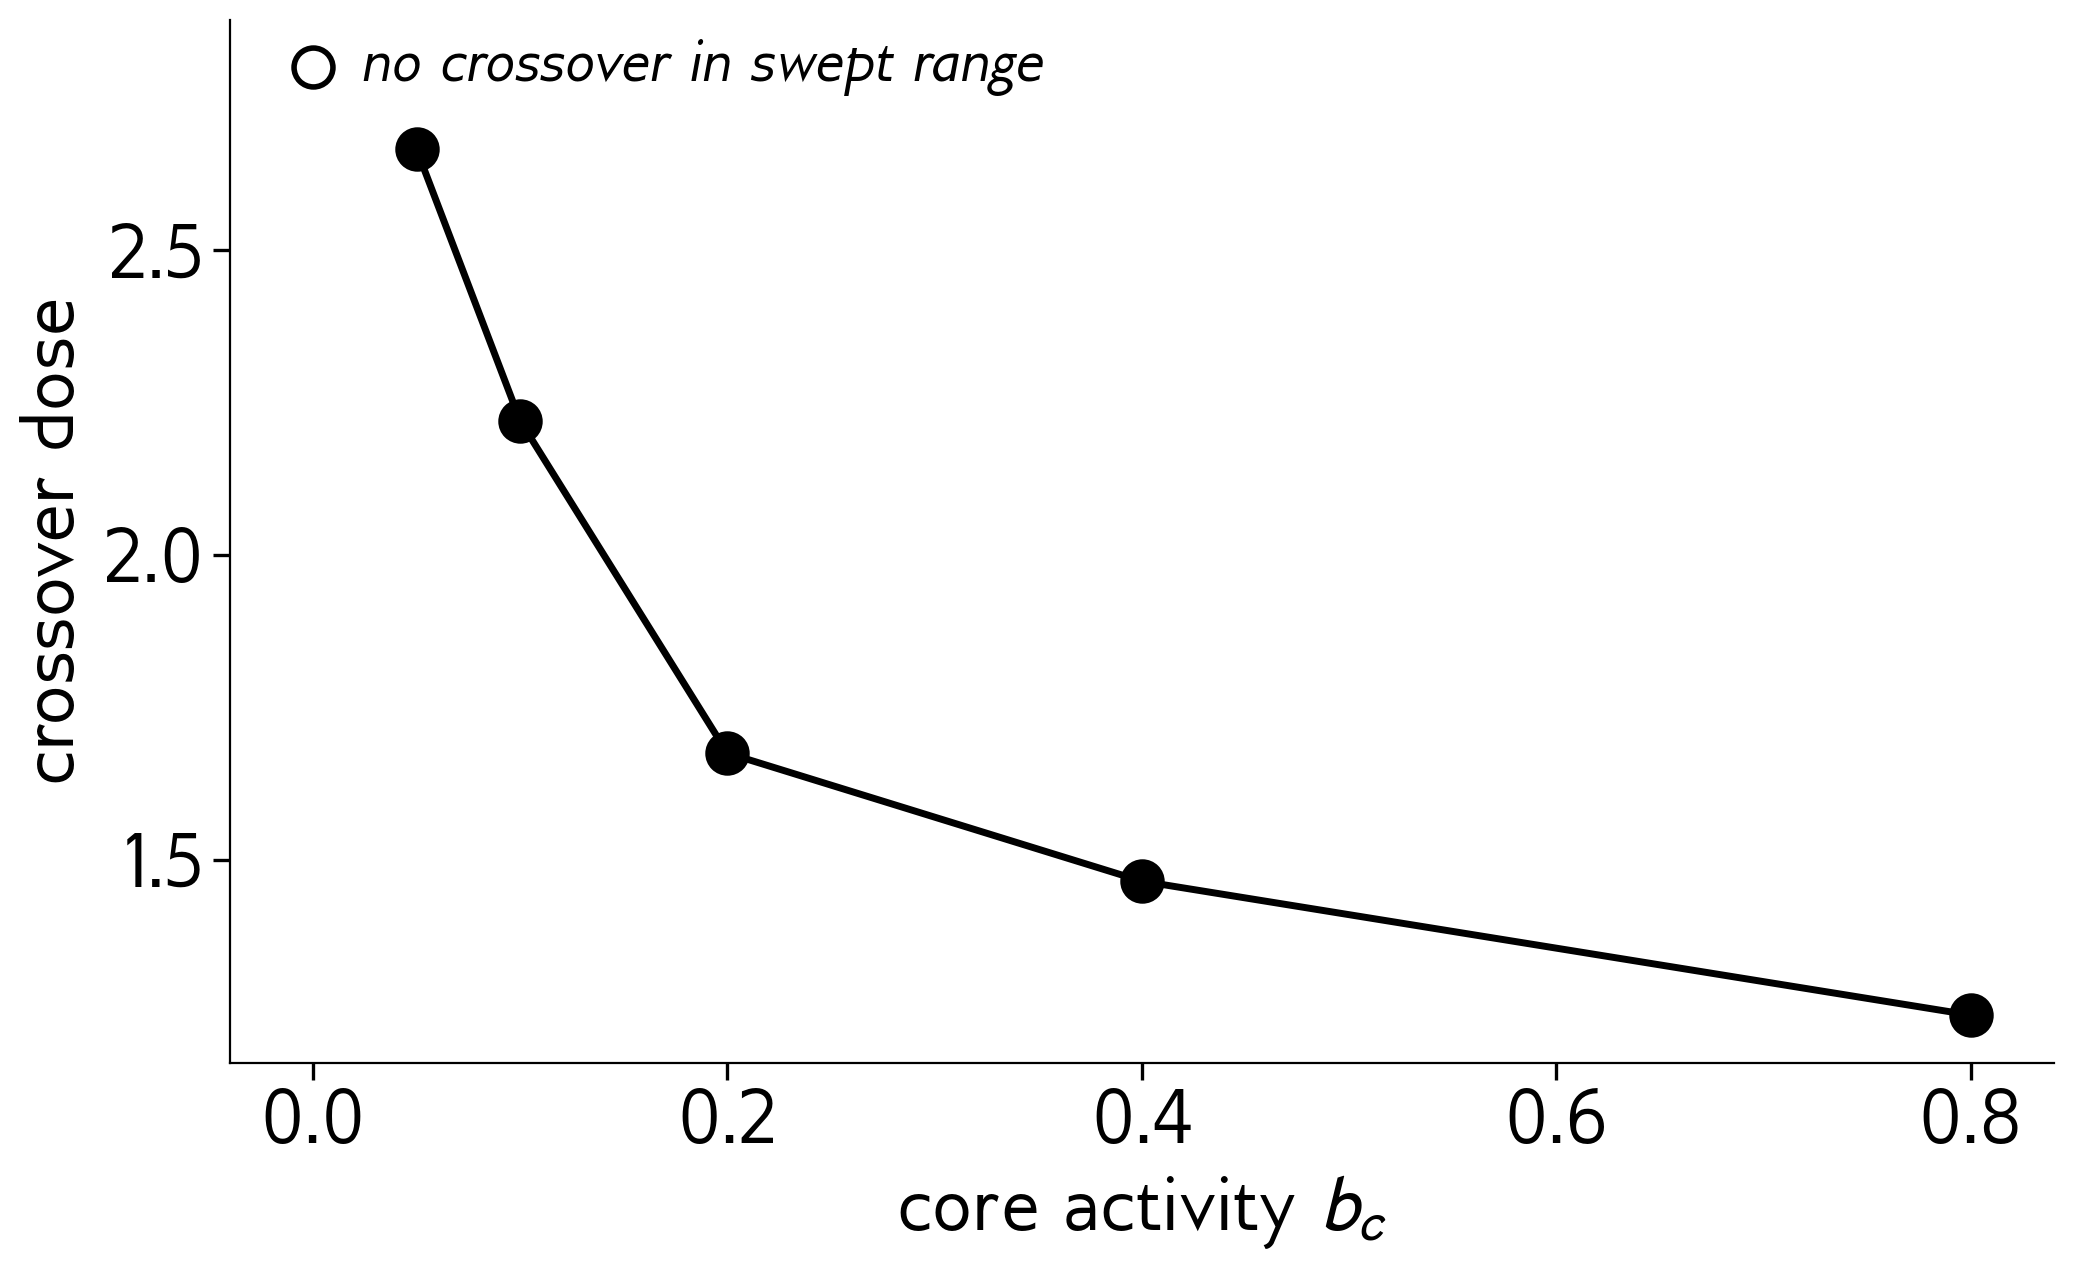
\includegraphics[width=0.65\textwidth]{crossover_vs_bc.png}
\caption{Crossover dose as a function of core activity $\bCore$, with
$l = 100$. The dormant case ($\bCore = 0$) has no crossover in the
swept range (open marker, top of plot). Every positive $\bCore$ has a
finite crossover, and the crossover dose drops monotonically as the
core gets more active---faster core turnover means the biofilm
overtakes the well-mixed reference at a lower dose.
\emph{Parameters}: same as Figure~\ref{fig:senscore}.}
\label{fig:xover_bc}
\end{figure}

The crossover dose drops sharply as the core wakes up, and then
levels off. Going from $\bCore = 0.05$ to $\bCore = 0.2$ pulls the
crossover from $\dEdge \approx 2.7$ down to $\dEdge \approx 1.7$;
going from $\bCore = 0.2$ to $\bCore = 0.8$ only pulls it further
down to $\dEdge \approx 1.25$. Once the core is active at all, the
crossover is firmly inside the swept dose range; the precise speed
of the core changes how easily the crossover is reached but does not
gate the qualitative effect.

\paragraph{Why the crossover moves with $l$ and $\bCore$.}
The shifts in Figures~\ref{fig:xover} and \ref{fig:xover_bc} both go
in the direction of \emph{more core activity earns an earlier
crossover}: a smaller $l$ leaves more cells in the active interior,
and a larger $\bCore$ makes each interior cell divide faster. Both
knobs increase the same quantity---the rate at which the protected
interior generates resistance mutations. Figure~\ref{fig:mechgrid}
makes the supply effect explicit, and exposes a second, weaker
effect that pushes the other way.

\begin{figure}[htbp]
\centering
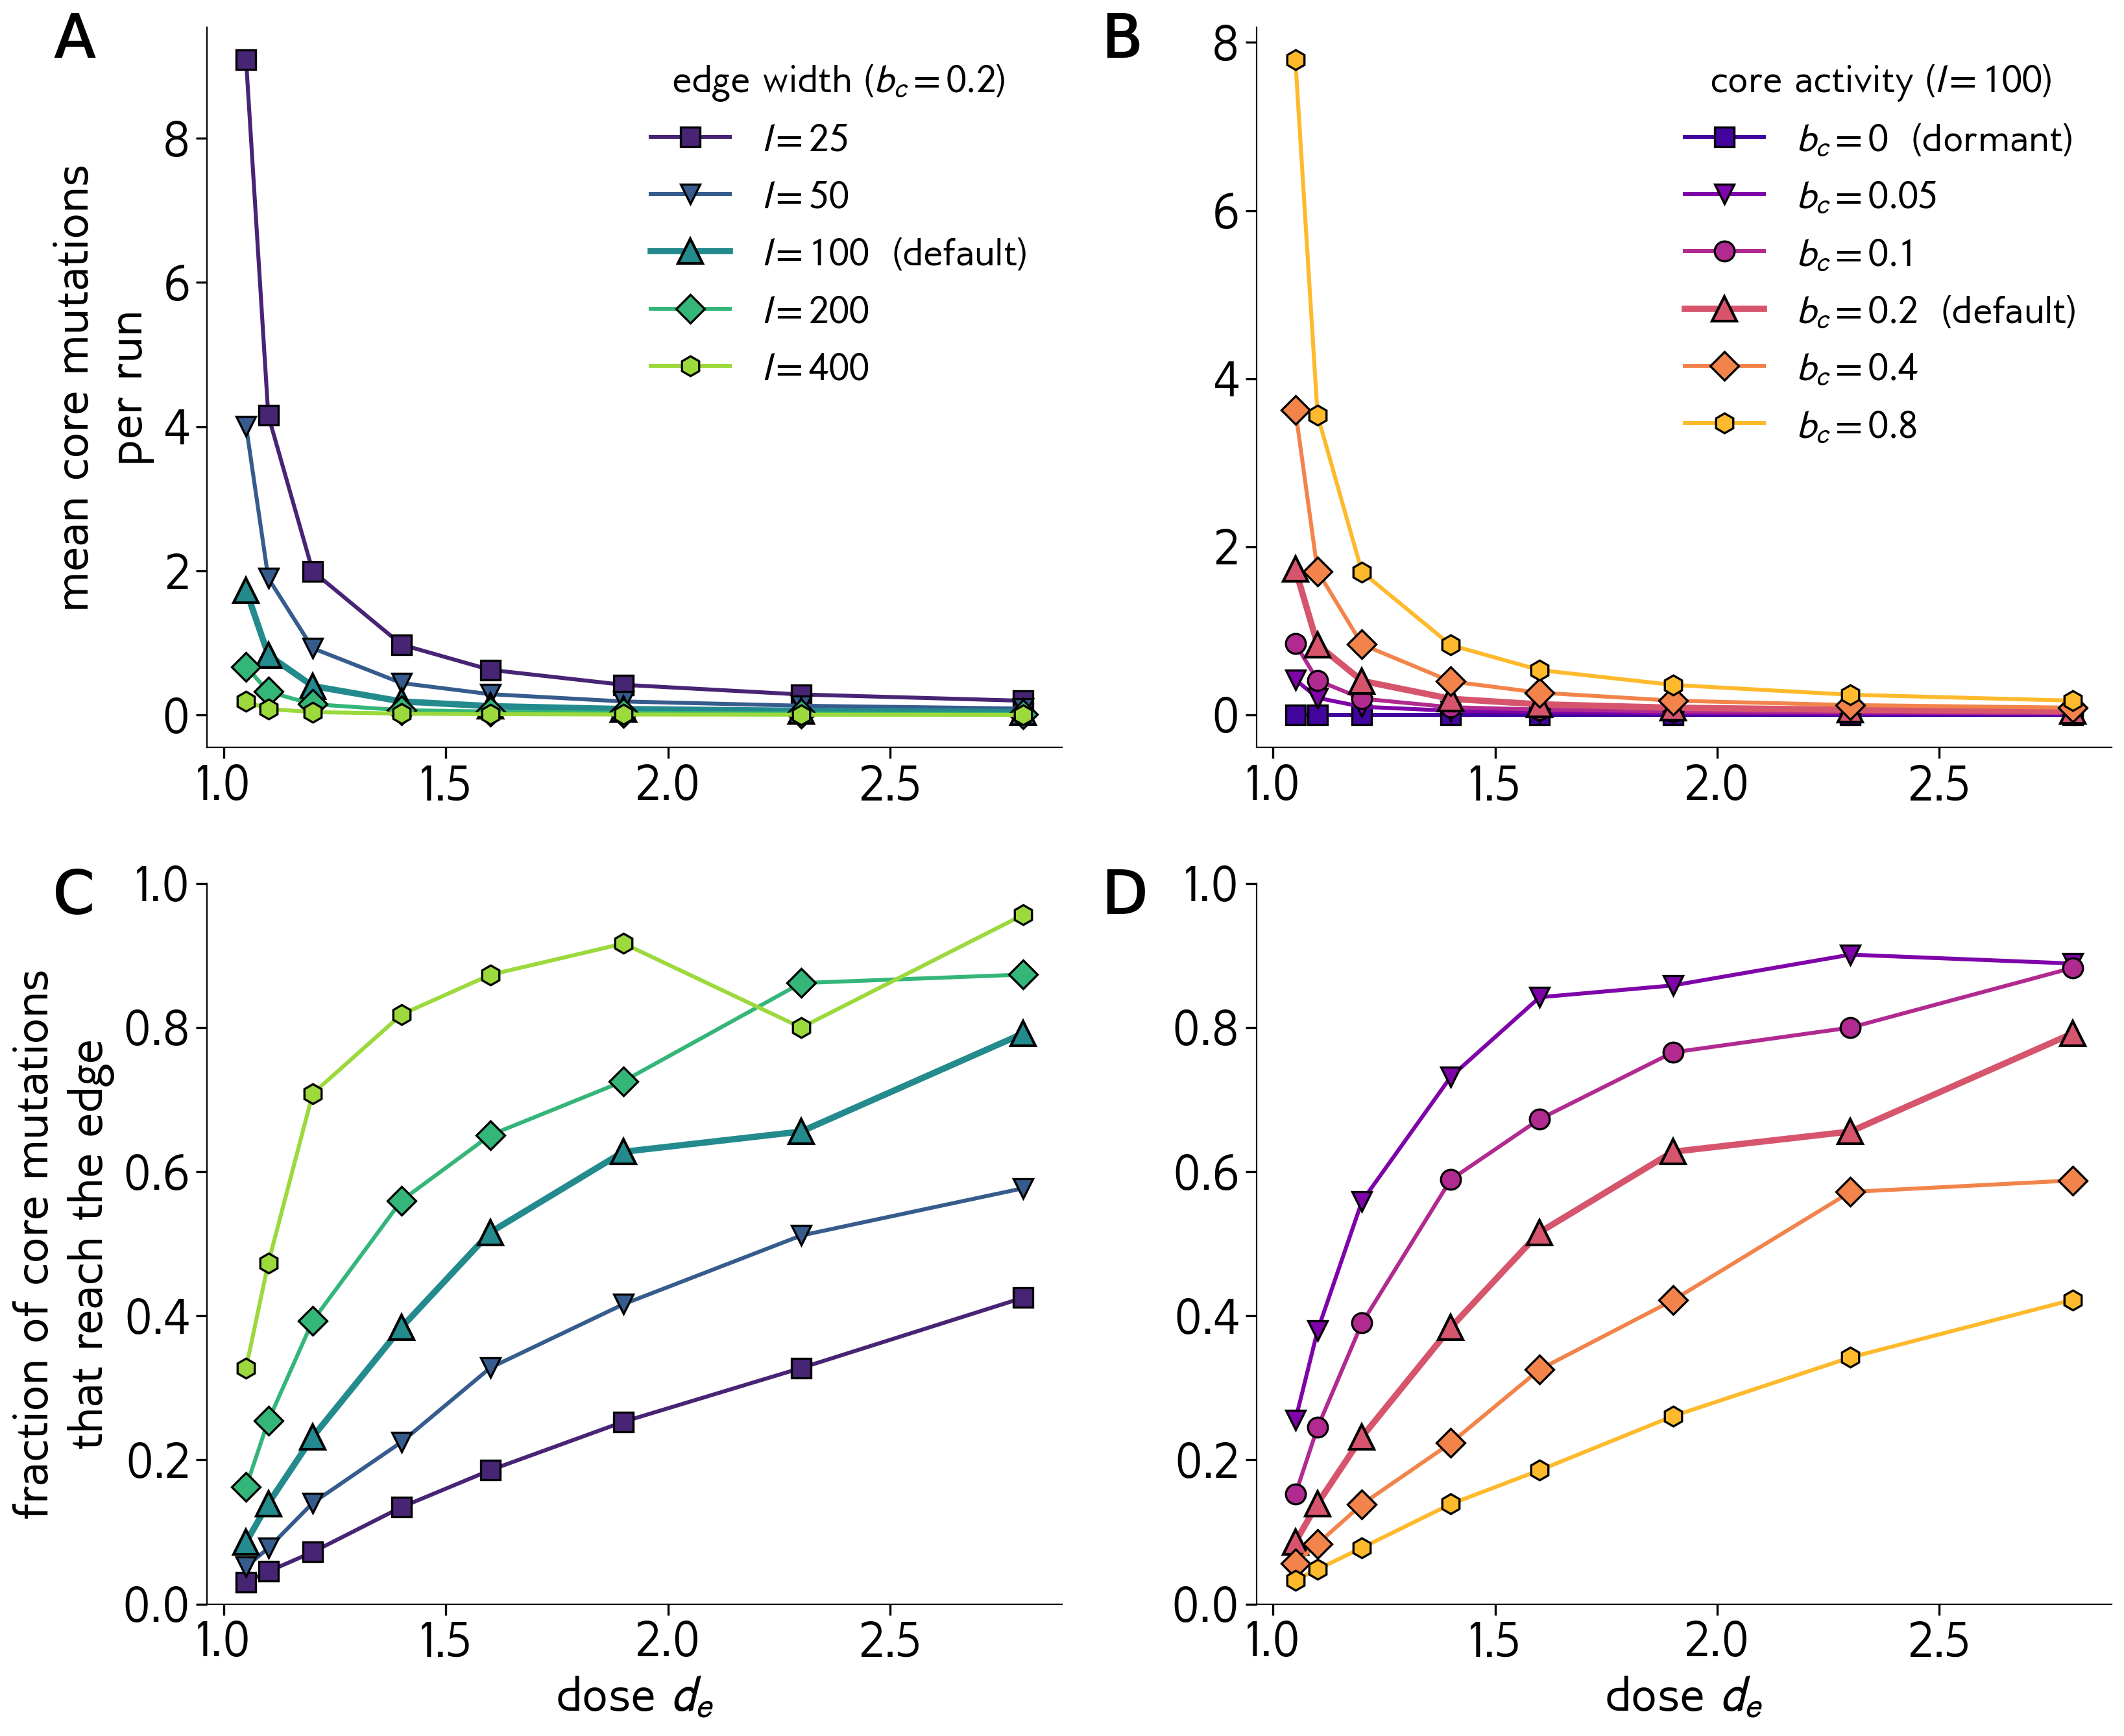
\includegraphics[width=0.97\textwidth]{mech_grid.png}
\caption{Two mechanism ingredients across the $l$ sweep (left column)
and the $\bCore$ sweep (right column). \textbf{Panels A, B}: mean
number of core-born resistance mutations per run, vs dose. Smaller
$l$ and larger $\bCore$ both make this number much larger---the
``supply bonus''. \textbf{Panels C, D}: fraction of those core-born
mutations that ever reach the edge (where they can grow). Smaller
$l$ \emph{lowers} the delivery fraction at every dose: the boundary
retreats at speed $s_e l$, so a thinner edge means a slower advance
and more time for drift to kill core lineages. Larger $\bCore$ also
lowers delivery: faster core turnover means more births competing
for the same lineage's offspring, so each lineage faces more drift
pressure. \emph{Parameters}: $N_0 = 1000$, $\mu = 10^{-4}$; left
column at $\bCore = 0.2$, right column at $l = 100$; each point
aggregates 5{,}000 runs.}
\label{fig:mechgrid}
\end{figure}

Both supply and delivery shift in opposite directions when we tune
$l$ or $\bCore$. A smaller $l$ produces a lot more mutations but
delivers a smaller fraction of them; a larger $\bCore$ produces more
mutations but delivers fewer. In both cases the supply effect wins
by a large margin---the supply curves change by close to an order of
magnitude across the swept range, while the delivery fractions
change by a factor of two or three. The net effect is that
crossovers happen earlier when either knob is turned toward ``more
active core'', as we saw in Figures~\ref{fig:xover}
and~\ref{fig:xover_bc}.

\paragraph{What is the biofilm doing differently from well-mixed?}
Rescue requires two things: a population has to \emph{produce} a
resistance mutation, and that mutation has to \emph{take over} the
edge. These two ingredients can be measured separately, so we can
ask whether the biofilm differs from well-mixed in the rate at
which mutations appear, the rate at which appearing mutations
successfully establish, or both. Figure~\ref{fig:decomposition}
plots the two ingredients side by side.

\begin{figure}[htbp]
\centering
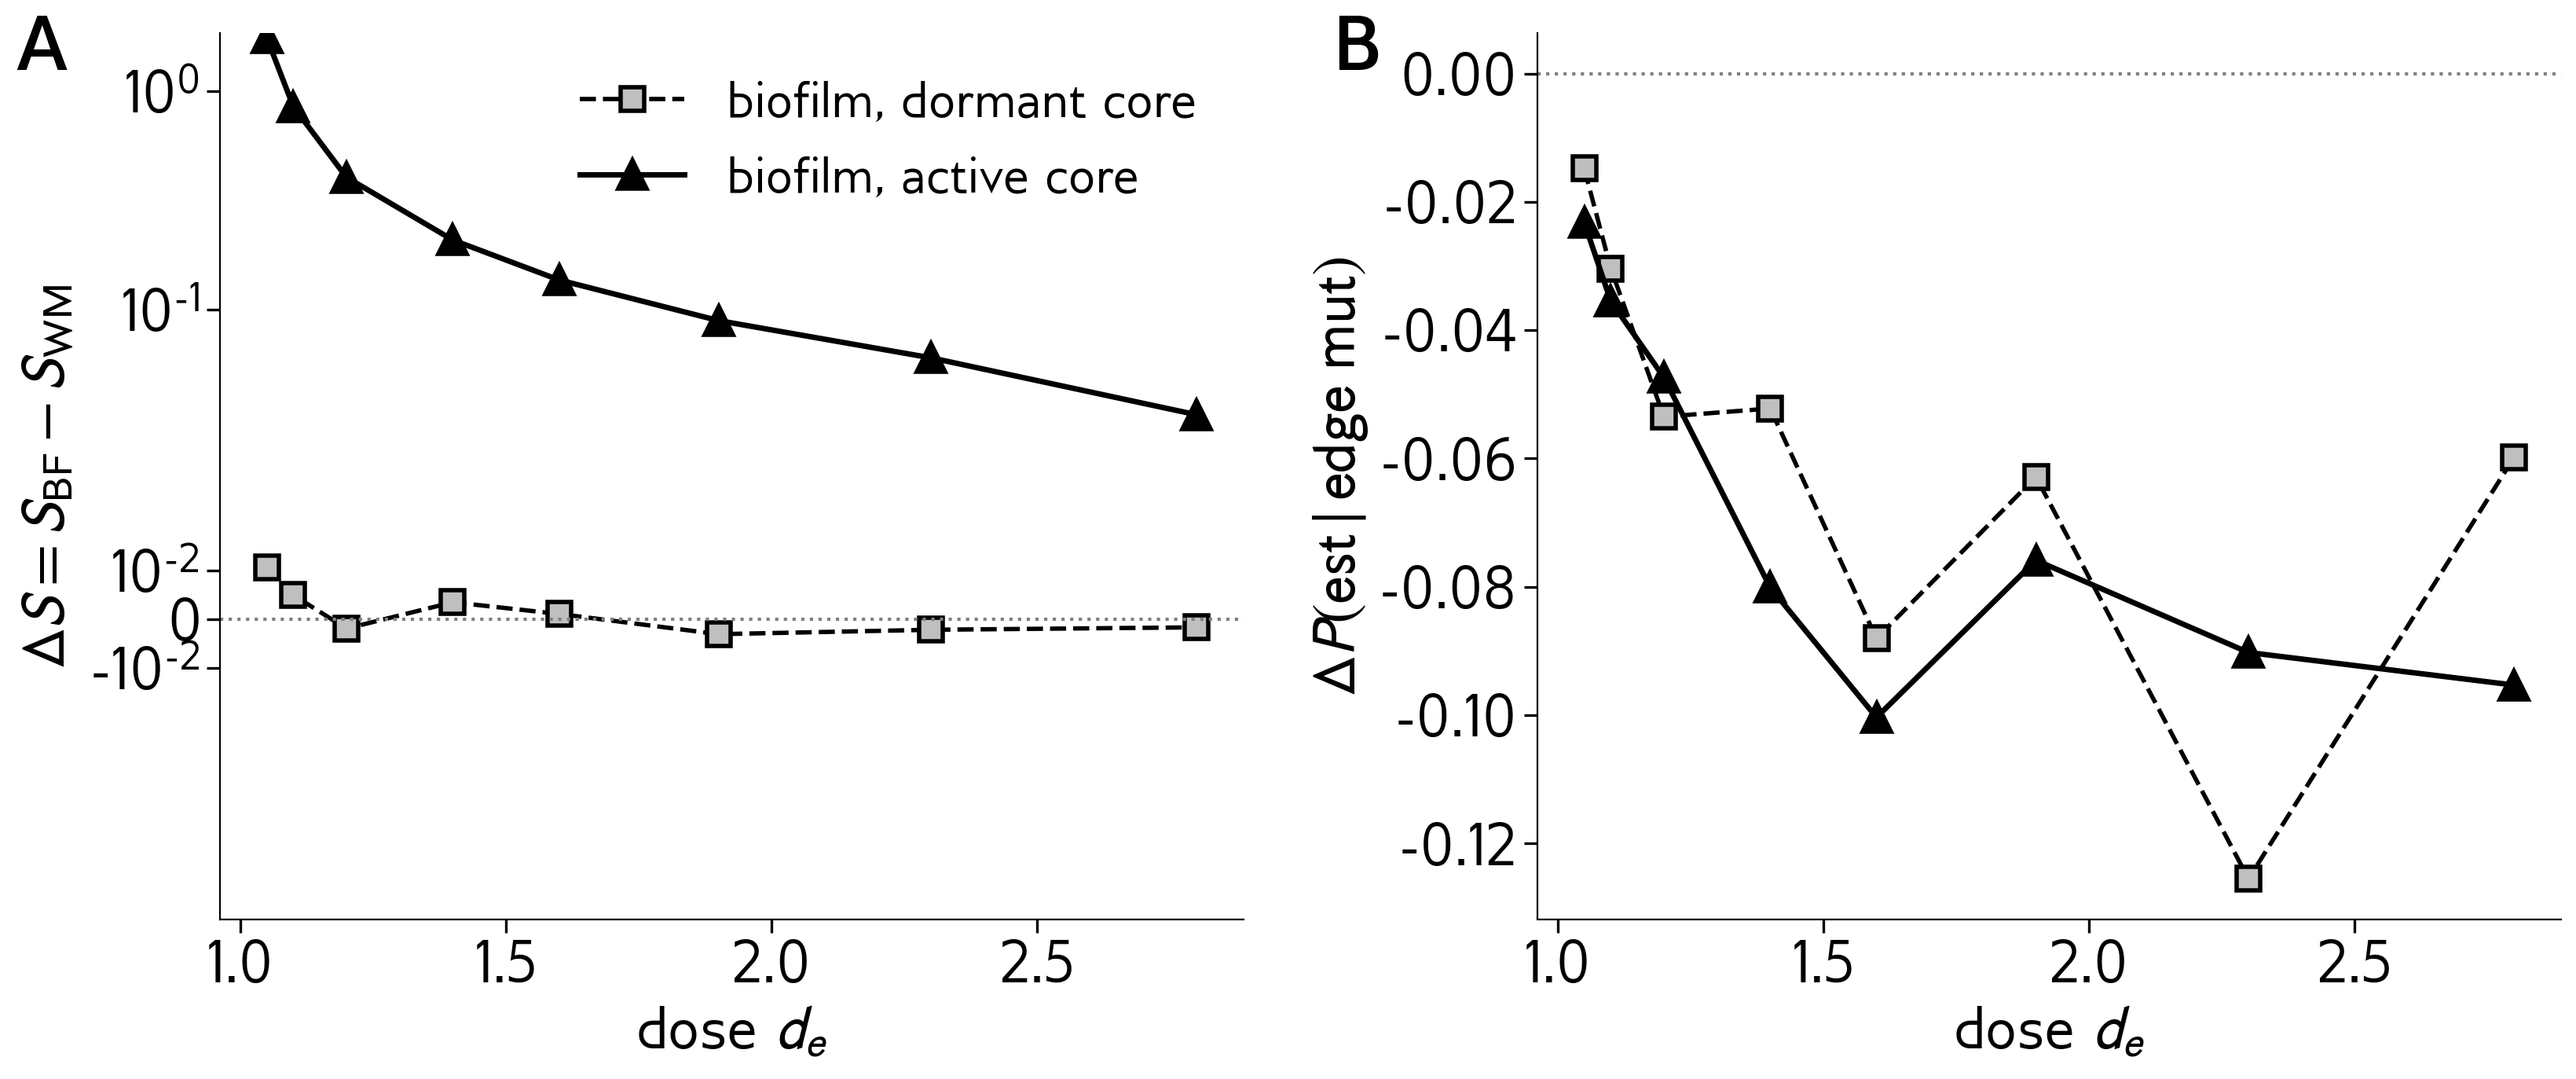
\includegraphics[width=0.97\textwidth]{decomposition.png}
\caption{\textbf{A}: Mean number of resistance mutations produced per
simulation run, across dose. The well-mixed and biofilm-dormant curves
overlap almost exactly---an active core is what makes the biofilm
generate extra mutations. \textbf{B}: Per-mutation establishment
fraction, i.e.\ the fraction of edge-born mutations that grow to the
establishment threshold. The well-mixed reference is highest at every
dose; the biofilm-active is lowest at every dose. Each mutation in a
biofilm has a worse chance of taking over. \emph{Parameters}:
$N_0 = 1000$, $l = 100$, $\mu = 10^{-4}$; each point averages over
5{,}000 runs.}
\label{fig:decomposition}
\end{figure}

The two panels say opposing things.

\paragraph{Supply (Panel A): dormant biofilm and well-mixed lie on
top of each other.}
The well-mixed curve and the biofilm-with-dormant-core curve are
indistinguishable at every dose. Despite looking nothing alike
dynamically---one is a steadily shrinking ball of cells, the other
is a slowly draining biofilm with a protected interior---the two
produce the \emph{same number of resistance mutations} over their
entire lifetimes. This is a real prediction of the model, not a
coincidence, and Section~\ref{sec:supply} explains why. It also
gives the dormant biofilm a useful role: it has the same mutation
budget as well-mixed, so any difference in rescue rate between
those two must come from how mutations \emph{succeed}, not how
many appear.

An active core changes the picture: the active-core curve sits
about a factor of five above the other two. Those extra mutations
come from cell divisions in the protected interior---divisions
that the dormant biofilm and the well-mixed population do not
have.

\paragraph{Establishment (Panel B): biofilms pay a per-mutation
cost.}
The ordering reverses. The well-mixed curve is highest at every
dose; the active-core biofilm is lowest; the dormant biofilm sits
between them. Each individual resistance mutation in a biofilm is
roughly $1.5\times$ less likely to take over than the same mutation
in a well-mixed population. It is a real penalty, and it shows up
regardless of whether the core is active.

\paragraph{The two panels together explain Figures~\ref{fig:dosecurves}
and \ref{fig:sensl}.}
Rescue probability scales with the product of supply and
establishment.
\begin{itemize}[noitemsep,topsep=0pt]
    \item The dormant biofilm has the same supply as well-mixed but
    pays the per-mutation cost, so it loses at every dose. No
    crossover is possible.
    \item The active biofilm pays the same per-mutation cost but
    receives a $\sim 5\times$ supply bonus. Whether the bonus
    outweighs the cost depends on dose: at low dose the cost wins,
    at high dose the bonus wins. The crossover is the dose at which
    they balance.
\end{itemize}

This already tells the qualitative story. What remains is to explain
\emph{where each effect comes from}: why an active core produces
five times more mutations than well-mixed does, and why a biofilm
mutation is harder to establish. The next section
(Section~\ref{sec:supply}) handles the supply story---it is the
dominant effect and where the dose-dependent flip actually lives.
The per-mutation cost is treated more briefly later
(Section~\ref{sec:tax}); it is a roughly constant tax in the
background.

% ---------------------------------------------------------------------------
\section{Where the mutations come from: lifetime and supply}
\label{sec:supply}
% ---------------------------------------------------------------------------

The decomposition figure showed something surprising: well-mixed and the
biofilm with a dormant core produce the same total mutation supply,
even though the two populations look very different over time. The
biofilm should live longer---it has a buffered interior. Why doesn't a
longer lifetime translate into more mutations? And separately, where
does an active core's roughly five-fold supply bonus actually come
from? Both questions are best answered by looking at how the population
moves through time. Figure~\ref{fig:trajectory} shows the two
trajectories with mutations turned off, so the curves are pure
wild-type decline.

\begin{figure}[htbp]
\centering
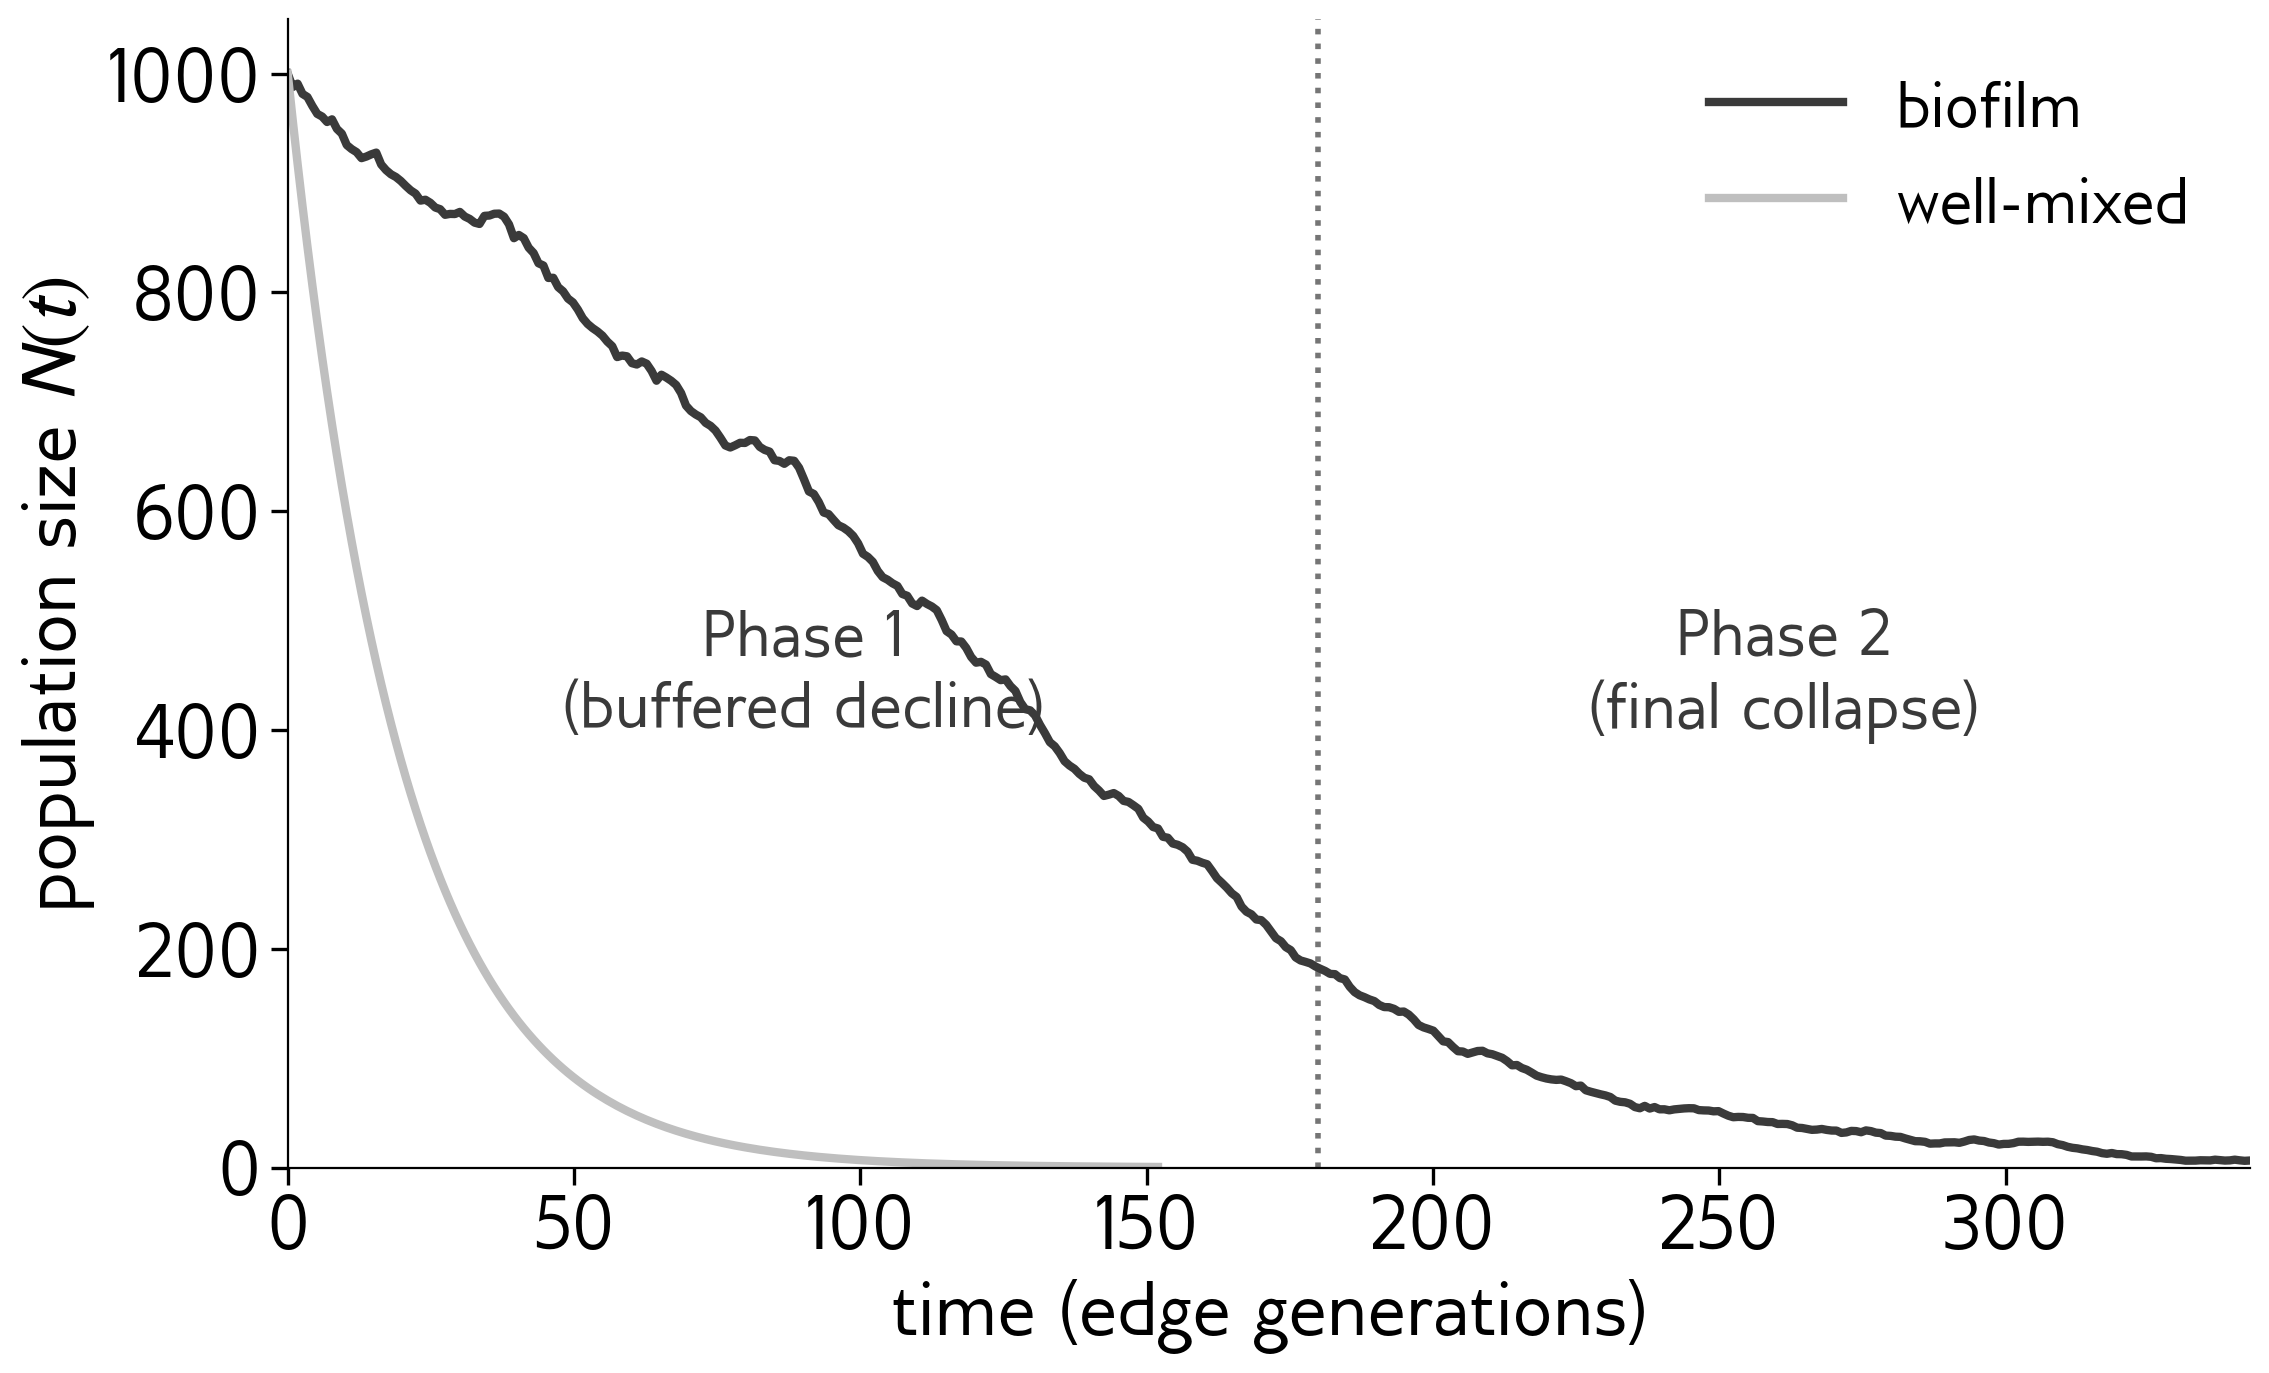
\includegraphics[width=0.85\textwidth]{trajectory.png}
\caption{Population size $N(t)$ for the biofilm and the well-mixed
reference, at $\dEdge = 1.05$ with mutations disabled. The biofilm
declines linearly during Phase 1 (the core feeds replacement cells
into the edge), then exponentially during Phase 2 (the core is
exhausted). The well-mixed population declines exponentially
throughout. The two curves have very different shapes but the same
area underneath. \emph{Parameters}: $N_0 = 1000$, $l = 100$,
$\bCore = 0.2$, $\mu = 0$ (no mutations, so what we see is the pure
wild-type decline). Biofilm curve is the mean of 20 independent
runs; well-mixed curve is the analytical exponential decay.}
\label{fig:trajectory}
\end{figure}

\paragraph{Two shapes, one area.}
The biofilm survives roughly twice as long as the well-mixed
population, but it is at a smaller size for most of that extra time.
Concretely: during Phase 1, only the $l = 100$ edge cells experience
the antibiotic, so only those $l$ cells contribute to the net decline.
The total population falls linearly at rate $s_e l$ until the core is
gone, which takes $T_1 = (N_0 - l)/(s_e l)$ time units. Once the core
is exhausted, the remaining $l$ cells decay exponentially at rate
$s_e$ for another $\sim \ln(l)/s_e$ time units before extinction.

What controls mutation supply is not lifetime; it is total cell-time,
$\int N(t)\, dt$---the area under the curve. Each cell-time unit
allows $b_e \mu$ wild-type birth-mutations on average, and the
mutations are what the rescue race depends on. The well-mixed
population is also dying exponentially at rate $s_e$, so its total
cell-time is $\int_0^\infty N_0 e^{-s_e t}\, dt = N_0 / s_e$. For the
biofilm-with-dormant-core, only the edge contributes to mutation
supply, and the edge holds $l$ cells for time $T_1$ and then decays
exponentially. Its total edge cell-time works out to
\[
l \cdot \frac{N_0 - l}{s_e l} \,+\, \frac{l}{s_e}
\;=\; \frac{N_0 - l}{s_e} + \frac{l}{s_e}
\;=\; \frac{N_0}{s_e}.
\]
Same integral, despite very different shapes. This is the clean
prediction behind the curves overlapping in Figure~\ref{fig:decomposition}A.
A spatial structure that stretches a population's lifetime without
adding any extra dividing cells does not change the mutation budget.

\paragraph{Where the active core's bonus comes from.}
An active core changes the picture by adding dividing cells---ones
that are not contributing to the antibiotic-driven decline, but that
are still hosting birth events. During Phase 1, core cells divide at
rate $b_c$ each, and there are roughly $(N_0 - l)/2$ of them on
average over the Phase 1 window. Their integrated cell-time is
\[
\text{core cell-time} \;\approx\; \frac{(N_0 - l)^2}{2 s_e l},
\]
and the rate at which they produce mutations is $b_c \mu$ per cell.
With our defaults at low dose ($N_0 = 1000$, $l = 100$, $s_e = 0.05$,
$\mu = 10^{-4}$), the edge contributes roughly two mutations per run
and the core, at $b_c = 0.8$, contributes another five or six. The
biofilm with an active core therefore produces roughly three times
the supply of the well-mixed reference, in line with what
Figure~\ref{fig:decomposition}A shows.

The active core's contribution is purely additive: it sits on top of
the same edge supply that the well-mixed population also has. The
biofilm does not gain or lose from the conveyor belt itself; it gains
extra mutations exclusively because of the metabolic activity in the
interior. A faster core means more core births, more mutations, and a
bigger bonus.

\paragraph{So the supply story is settled.}
The biofilm-with-dormant-core and the well-mixed reference produce
the same number of mutations because they share the same total edge
cell-time, even though their lifetime profiles differ. A biofilm with
an active core produces more mutations because its core cells are
also dividing.

But supply alone does not determine rescue. The next section asks the
follow-up question: of the extra mutations that an active core
produces, how many are useful? It turns out most of them are not.

% ---------------------------------------------------------------------------
\section{Why only some of those mutations matter}
\label{sec:delivery}
% ---------------------------------------------------------------------------

The previous section showed that an active core produces several
extra resistance mutations per run. But producing a mutation is not
the same as using it. A resistant cell only matters for rescue if it
ends up in the edge---where it can grow under the antibiotic
selection that gives it a survival advantage. A resistant cell stuck
in the shielded core does nothing, because there is no selection
there. So the question for this section is: of all the extra
mutations an active core produces, how many actually make it out to
the edge in time to matter?

\paragraph{Why mutations get stuck in the core.}
Resistant cells in the core grow and die at the same rate
($b_c = d_c$), so on average their numbers do not change. But ``on
average'' hides what actually happens. A lineage that starts as a
single cell mostly does not grow at all; it just bounces around
randomly in size due to chance birth and death events, and eventually
the bouncing brings it back to zero. This is sometimes called drift,
and it is the default fate of a neutral lineage starting from one
cell. To put numbers on it: a single neutral cell goes extinct with
probability one given enough time.

For the lineage to escape this default fate, it has to get out of the
core before bad luck eliminates it. The way out is mechanical: the
biofilm is shrinking from the outside in, and the boundary between
core and edge retreats inward at speed $s_e l$ per unit time. When
the boundary passes over a core cell, that cell is reclassified as an
edge cell. The lineage is now in the drug-exposed edge, where its
resistance is worth something.

The wait between when a mutation is born and when the boundary
catches up to it depends on the dose. At low dose the boundary
retreats slowly, so the wait can be very long, giving the lineage a
lot of time to die from drift before delivery. At high dose the
boundary races inward, sweeping up surviving lineages before drift
gets a chance.

\paragraph{Watching it happen (Figure~\ref{fig:kymograph}).}
Figure~\ref{fig:kymograph} is a space-time picture of one such
core-delivery rescue. Each row shows the state of the biofilm at one
moment in time (time runs downward on the y-axis); each column shows
one cell position, with the deep interior at the left and the outer
surface at the right. Grey is wild-type core, tan is wild-type edge,
blue is a resistant lineage. The black lines mark the inner edge
of the core (left line) and the outer surface (right line). Both
retreat leftward over time as the biofilm shrinks.

\begin{figure}[htbp]
\centering
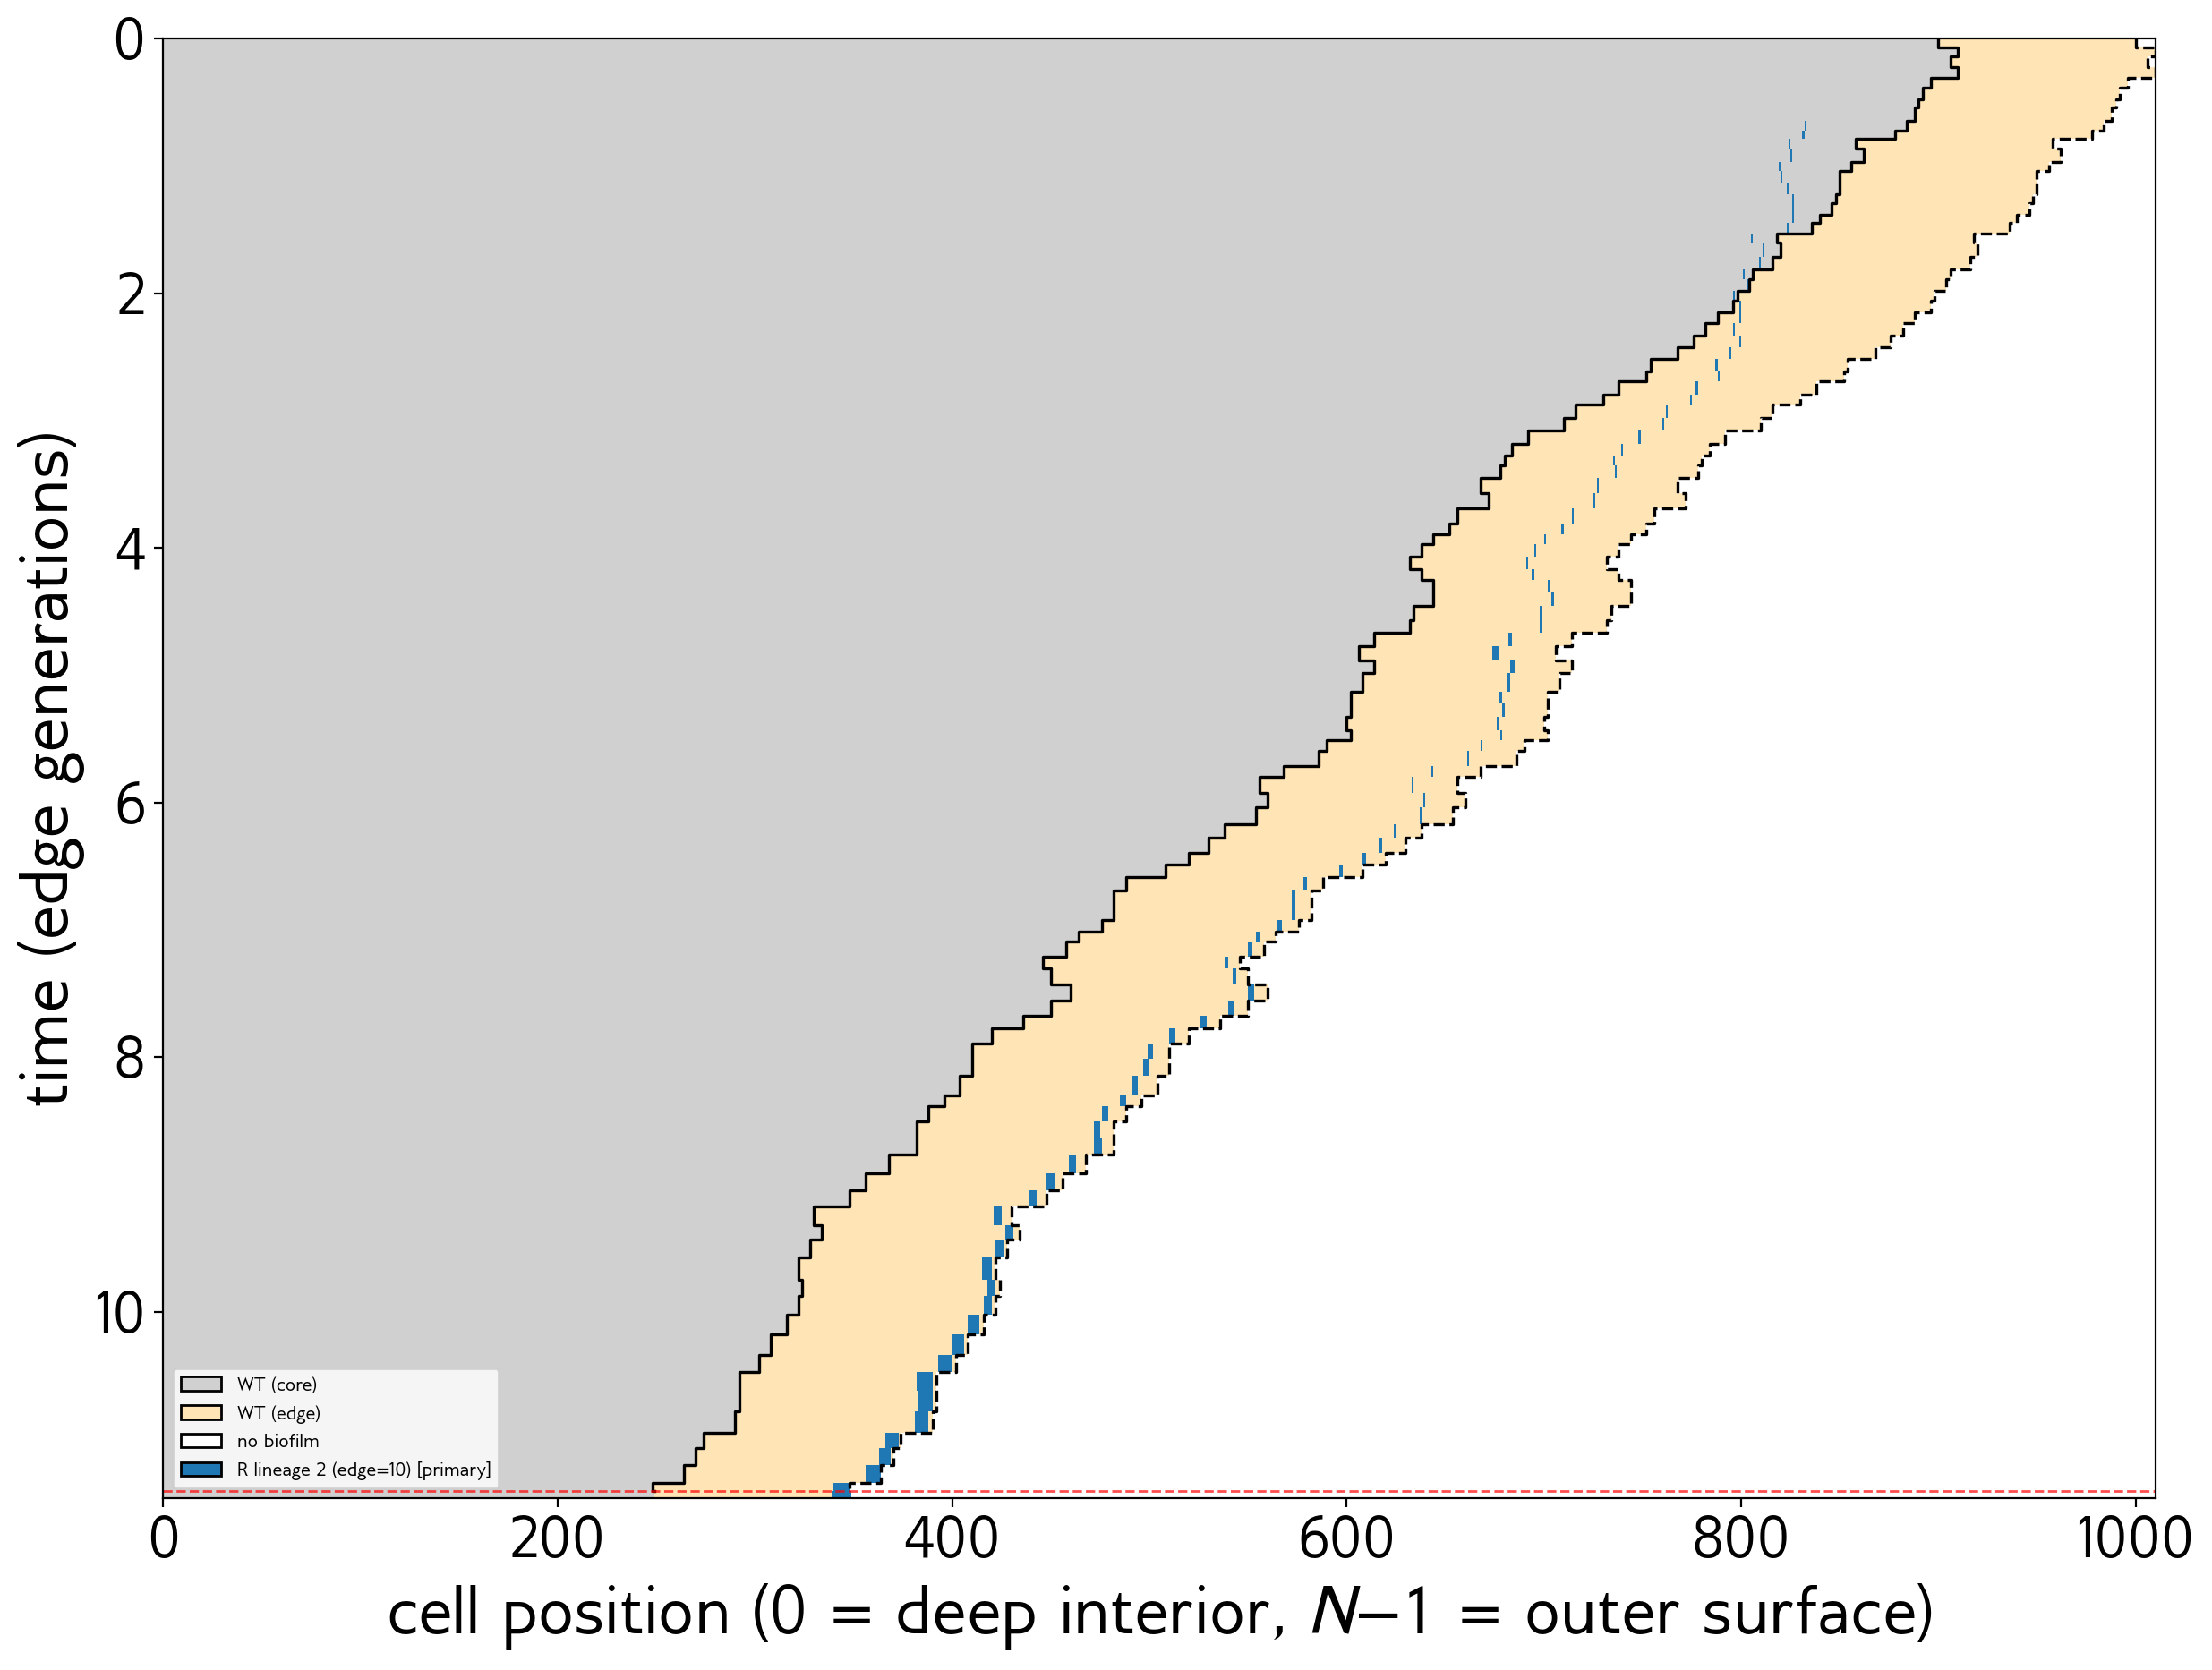
\includegraphics[width=0.9\textwidth]{kymograph_core_rescue.png}
\caption{A core-delivery rescue. The resistant lineage (blue) appears
in the shielded interior around position 800 at time $t \approx 0.7$.
It does not grow much during its time in the core (where neither WT
nor R has a selection advantage), but it survives. The boundary
between core and edge---the upper-left black line---retreats inward
toward the lineage. Around $t \approx 9$ the boundary reaches it and
the resistant cells become edge cells. They then grow rapidly under
antibiotic pressure, and rescue is triggered at $t = 11.4$.
\emph{Parameters}: single simulation run at $\dEdge = 1.5$,
$N_0 = 1000$, $l = 100$, $\bCore = 0.2$, $\mu = 5 \times 10^{-4}$.
The mutation rate is higher than the default $10^{-4}$ used elsewhere,
chosen so that a clean core-delivery rescue appears in a tractable
seed scan; the mechanism does not depend on $\mu$.}
\label{fig:kymograph}
\end{figure}

The figure shows the mechanism: the resistant cell appears in the
core, sits there while bouncing around in size, gets reclassified
into the edge once the boundary reaches it, and then takes over.
Most of the action happens \emph{not} when the mutation is created,
but when it is delivered.

\paragraph{The aggregate signature (Figure~\ref{fig:delivery}A).}
Across many runs and many doses, the fraction of core-born resistant
lineages that ever reach the edge climbs sharply with dose. Panel A
of Figure~\ref{fig:delivery} plots this fraction. For a highly active
core ($b_c = 0.8$), the curve goes from about $5\%$ at our lowest
dose to about $40\%$ at our highest dose---roughly an eightfold
range. At the lower core activity ($b_c = 0.2$, the default in the
main sweep), more lineages make it out at every dose, but the
qualitative trend is the same. (The two values differ because faster
core turnover means more births, so each lineage has more competing
births nearby, but the underlying drift mechanism is identical.)

\begin{figure}[htbp]
\centering
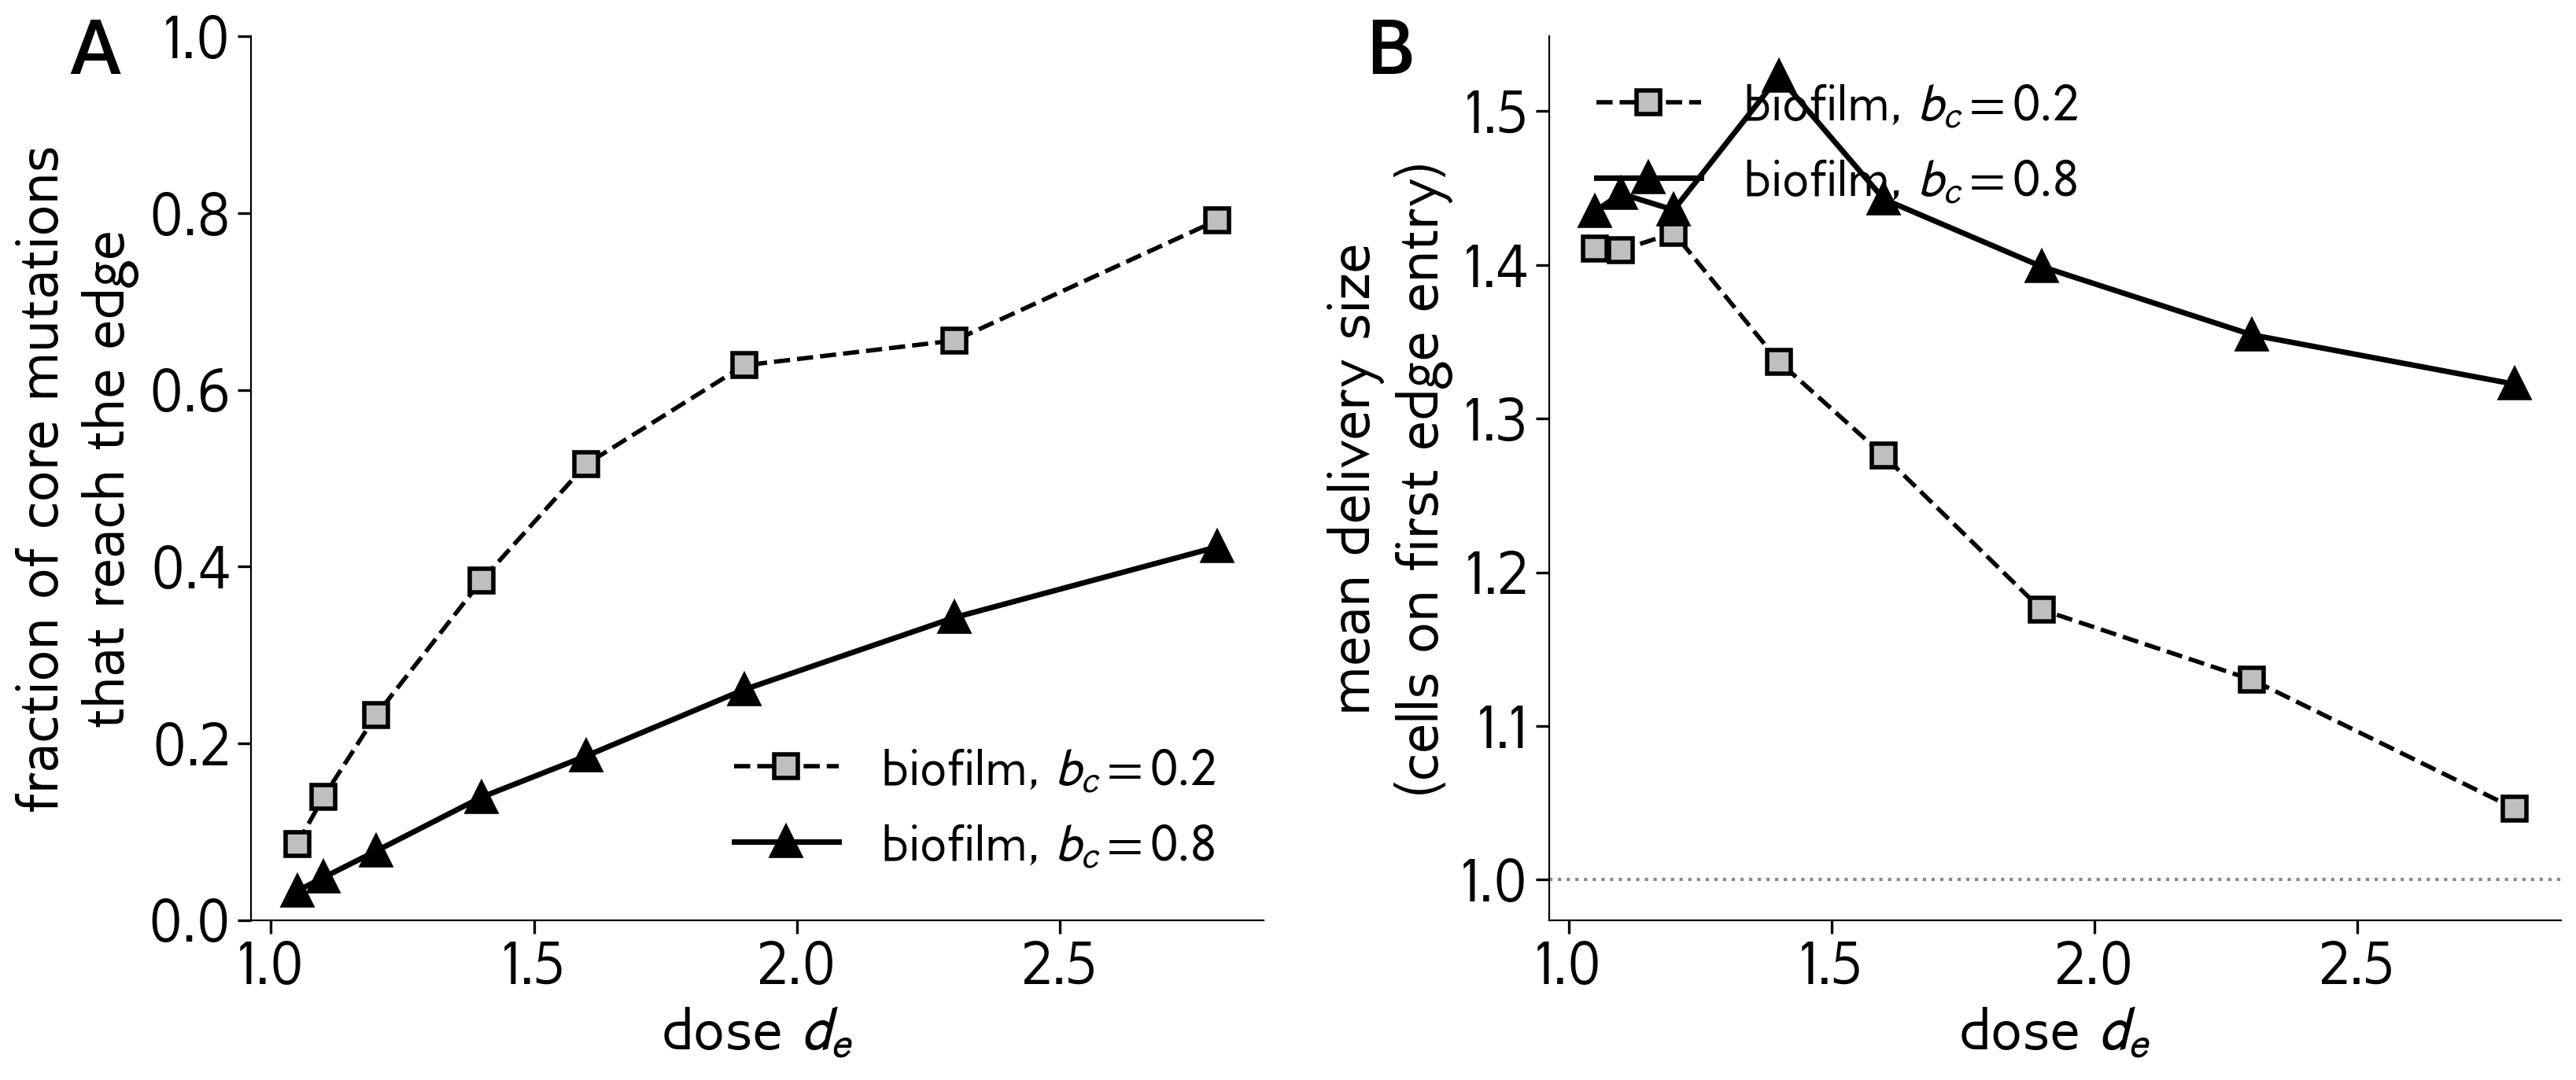
\includegraphics[width=0.97\textwidth]{delivery.png}
\caption{\textbf{A}: Fraction of core-born resistant lineages that
ever reached the edge, plotted against dose, at two core activity
levels. Both curves rise strongly with dose. At low dose almost all
the core's extra mutations are lost before they can be useful; at
high dose a much larger fraction reaches the edge. \textbf{B}:
Average size of a delivered lineage at the moment it first enters
the edge. A value of $1$ (dotted line) means single-cell arrivals.
Delivered lineages tend to arrive as small clumps of about
$1$--$1.5$ cells. Counterintuitively, the clumps are slightly
\emph{larger} at low dose, because the few lineages that survive the
long wait have had more time to also grow. \emph{Parameters}:
$N_0 = 1000$, $l = 100$, $\mu = 10^{-4}$; each point aggregates all
core-born mutations from 5{,}000 independent runs.}
\label{fig:delivery}
\end{figure}

\paragraph{A small secondary effect: arrivals come as clumps, not
single cells (Figure~\ref{fig:delivery}B).}
There is a second, weaker effect worth flagging. When a core lineage
sits in the core for a long time before being delivered, it is not
just drifting toward extinction---it can also drift toward larger
sizes by the same coin flips. Conditional on \emph{not} dying out,
the surviving lineage tends to grow a bit. So lineages that wait a
long time and survive arrive at the edge not as a single cell but as
a small clump of cells. Panel B of Figure~\ref{fig:delivery} shows
this: arrival sizes average $1.5$ cells at low dose (where the wait
is long) and drop to $1.0$--$1.3$ at high dose (where the wait is
short). A clump of cells has a slight edge over a single cell because
each cell is an independent chance to escape early-extinction drift,
but the effect is modest (a factor of $\sim 1.5$ in clump size, not
an order of magnitude), and it points the opposite direction from
the main delivery effect. The dominant story is the delivery
fraction.

\paragraph{Putting Sections~\ref{sec:supply} and \ref{sec:delivery}
together.}
An active core produces about five times the mutations of a
well-mixed population at any dose. At low dose, almost none of those
extra mutations get delivered into the edge in time, so they
contribute little to rescue. The biofilm has effectively the same
supply as well-mixed, and loses. At high dose, a substantial fraction
of the active core's extra mutations is delivered before drift
removes them, and the supply bonus finally translates into a rescue
advantage. The crossover between these regimes is the bar-plot flip.

% ---------------------------------------------------------------------------
\section{A small per-mutation tax}
\label{sec:tax}
% ---------------------------------------------------------------------------

\TODO{Brief treatment of the establishment penalty. Cite Panel B of
Fig~\ref{fig:decomposition}: BF mutations establish less often than
WM. Cause is two-part: (i) global N is preserved by the core during
Phase 1, lowering the density factor on R births; (ii) WT
competitors in the edge are continually replaced. Either way, the
result is a flat $\sim 20\%$ tax that the supply boost has to overcome.}

% --- OLD Track 1 SECTION (kept for reference, no longer in writeup) -------
\iffalse

The first track is the per-mutation deficit: every mutation in a
biofilm has a worse chance of taking over than the same mutation in a
well-mixed population. We argue this is caused by the conveyor belt,
specifically by what it does while the core is still present.

\paragraph{The mechanism.} While the core has cells in it, every WT
death in the edge pulls a fresh WT cell out of the core to take its
place. The edge therefore holds at a constant $l$ wild-type cells; the
antibiotic is killing WT, but the biofilm is instantly replacing every
one. A new R mutation that arises in the edge during this period faces
a wild-type majority that does not weaken over time. Compare this to
the well-mixed setting, where every WT death is just gone---the
competitive landscape eases for a new R lineage as the population
shrinks. In the biofilm, that easing never happens until the core is
exhausted.

This predicts a clean signature. Edge-born mutations should fall into
two distinct populations: those born during the buffered decline
(\textbf{Phase 1}, while the core exists and is supplying replacements)
and those born during the final collapse (\textbf{Phase 2}, after the
core has been consumed). Phase 1 mutations should be heavily
suppressed; Phase 2 mutations should look like well-mixed mutations,
because the relevant dynamics by that point are the same. The simulator
records, for each edge mutation, the time it appeared, so we can split
the two populations directly.

\paragraph{The signature is clean
(Figures~\ref{fig:phaselines}, \ref{fig:phasebars}).} The biofilm
Phase 1 establishment fraction sits well below the well-mixed reference
at every dose, by a factor of roughly $1.3$ to $1.6$. The Phase 2
fraction is at or above the well-mixed reference at every dose. Two
populations of edge mutations, born in the same physical biofilm under
the same antibiotic, behave completely differently---the only
difference is whether the core was still feeding the edge when they
arose. The mechanism is doing exactly what it should.

\begin{figure}[htbp]
\centering
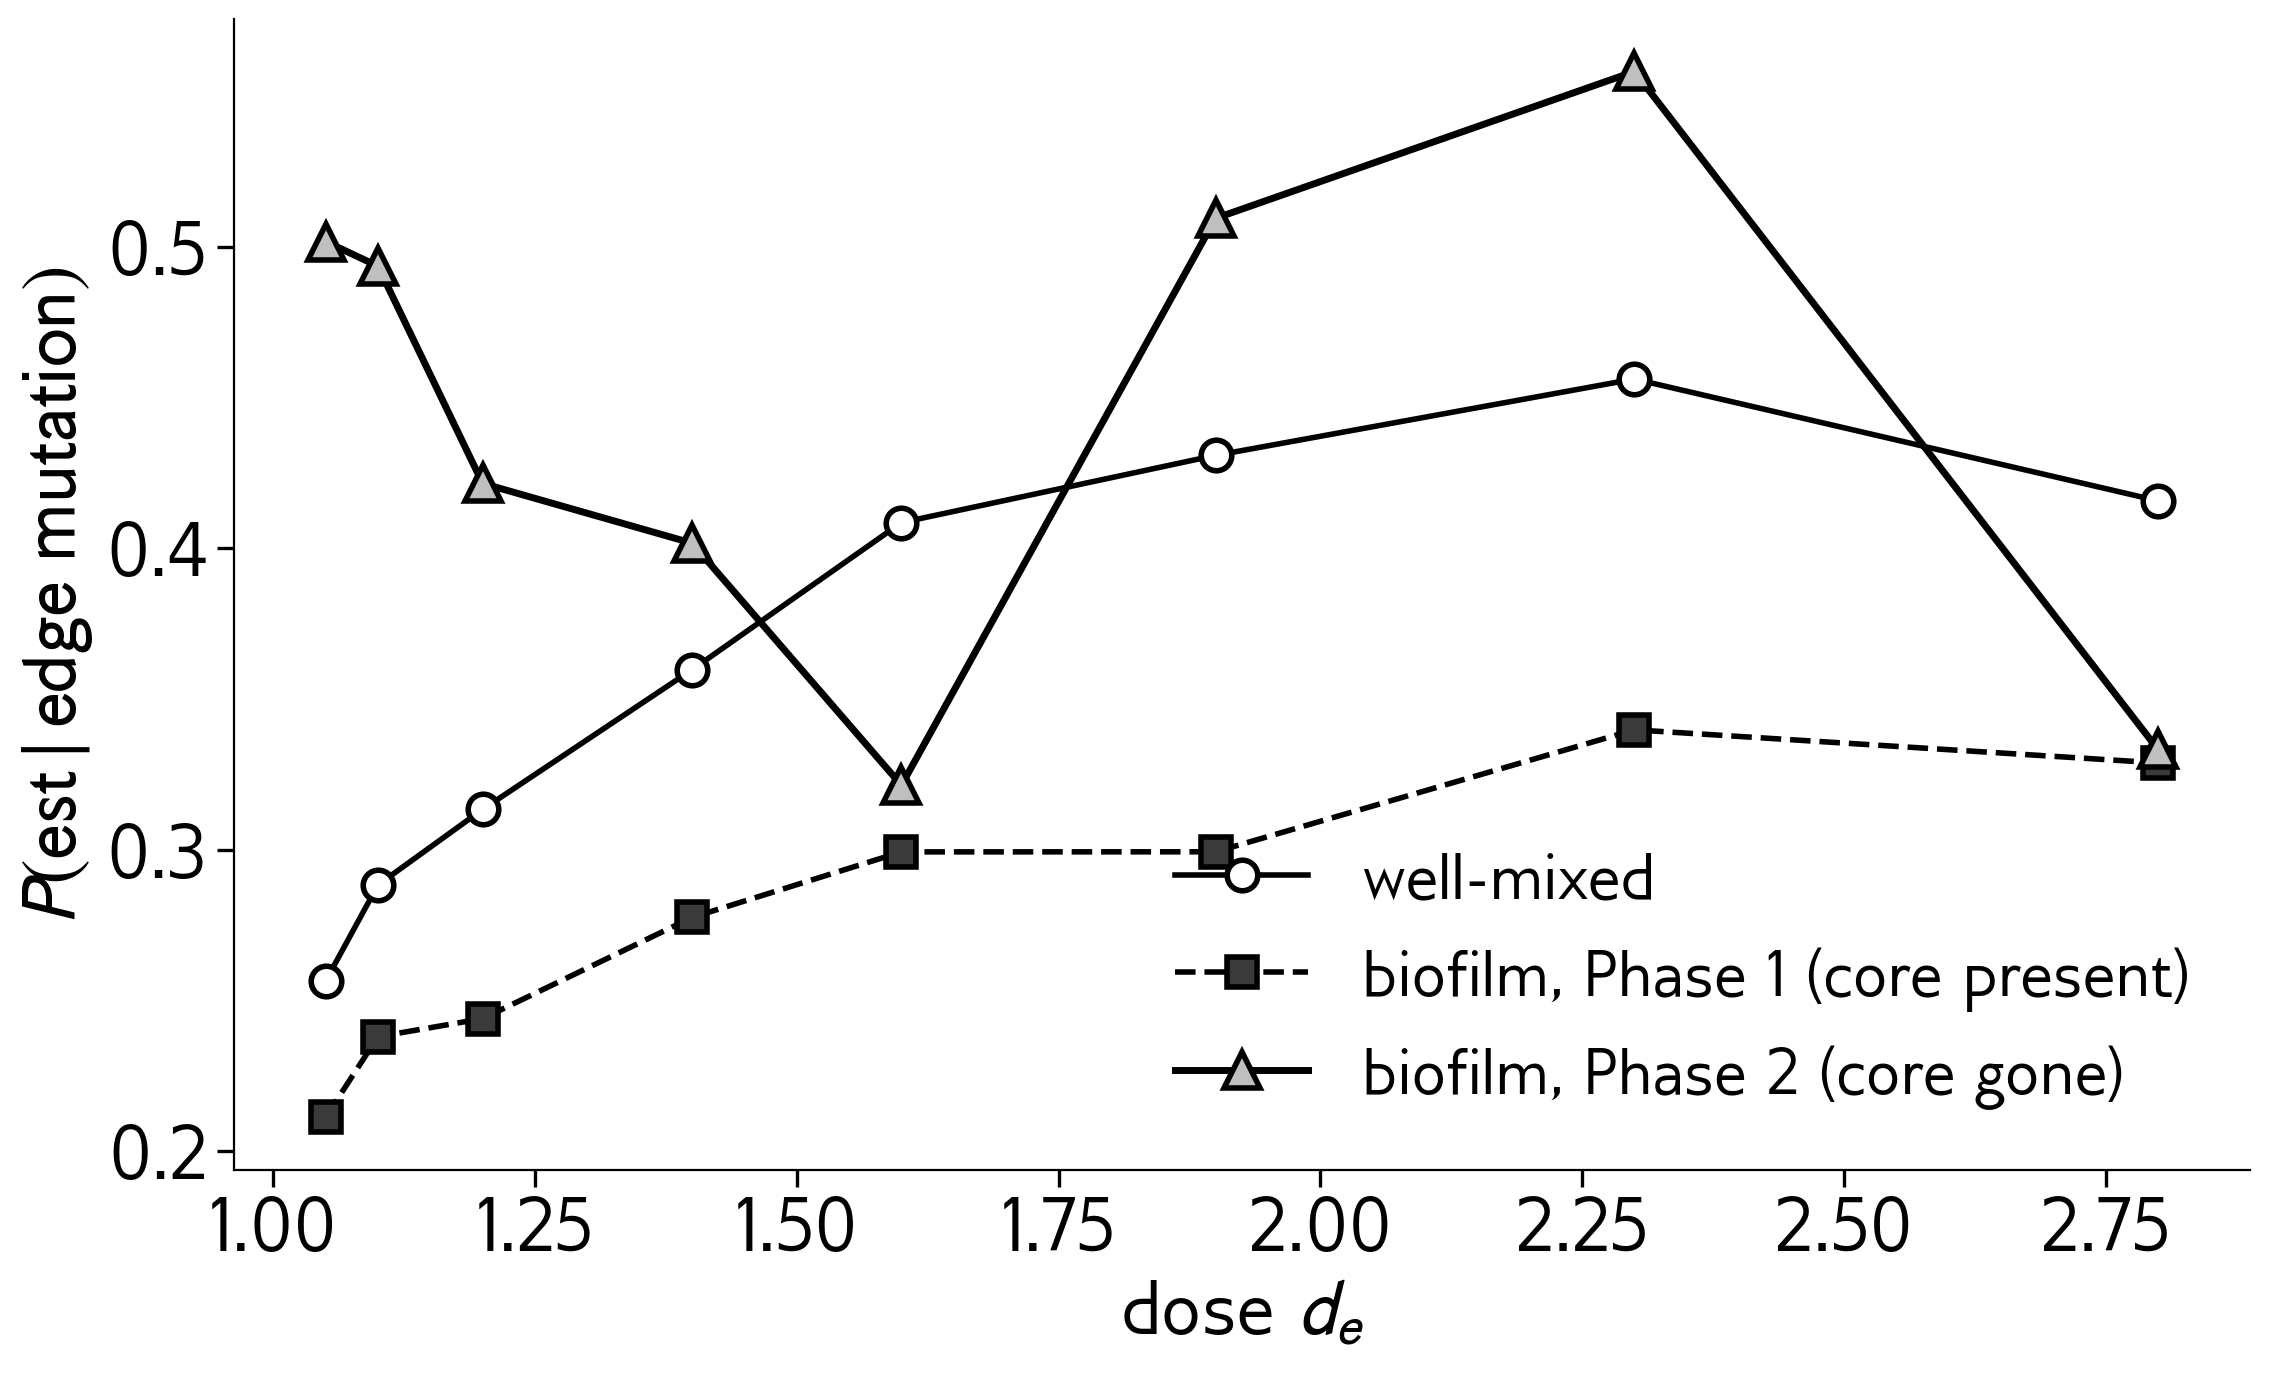
\includegraphics[width=0.85\textwidth]{estab_phase_lines.png}
\caption{Per-mutation establishment, edge-born mutations only, with the
biofilm split by birth phase. The biofilm Phase 1 curve (dashed
squares, the WT-resupply regime) is strictly below the well-mixed
reference at every dose. The biofilm Phase 2 curve (filled triangles,
after the core is gone) matches or exceeds the well-mixed reference.
The high-dose Phase 2 sample sizes are small ($n < 60$) and the curve
is noisy there.}
\label{fig:phaselines}
\end{figure}

\begin{figure}[htbp]
\centering
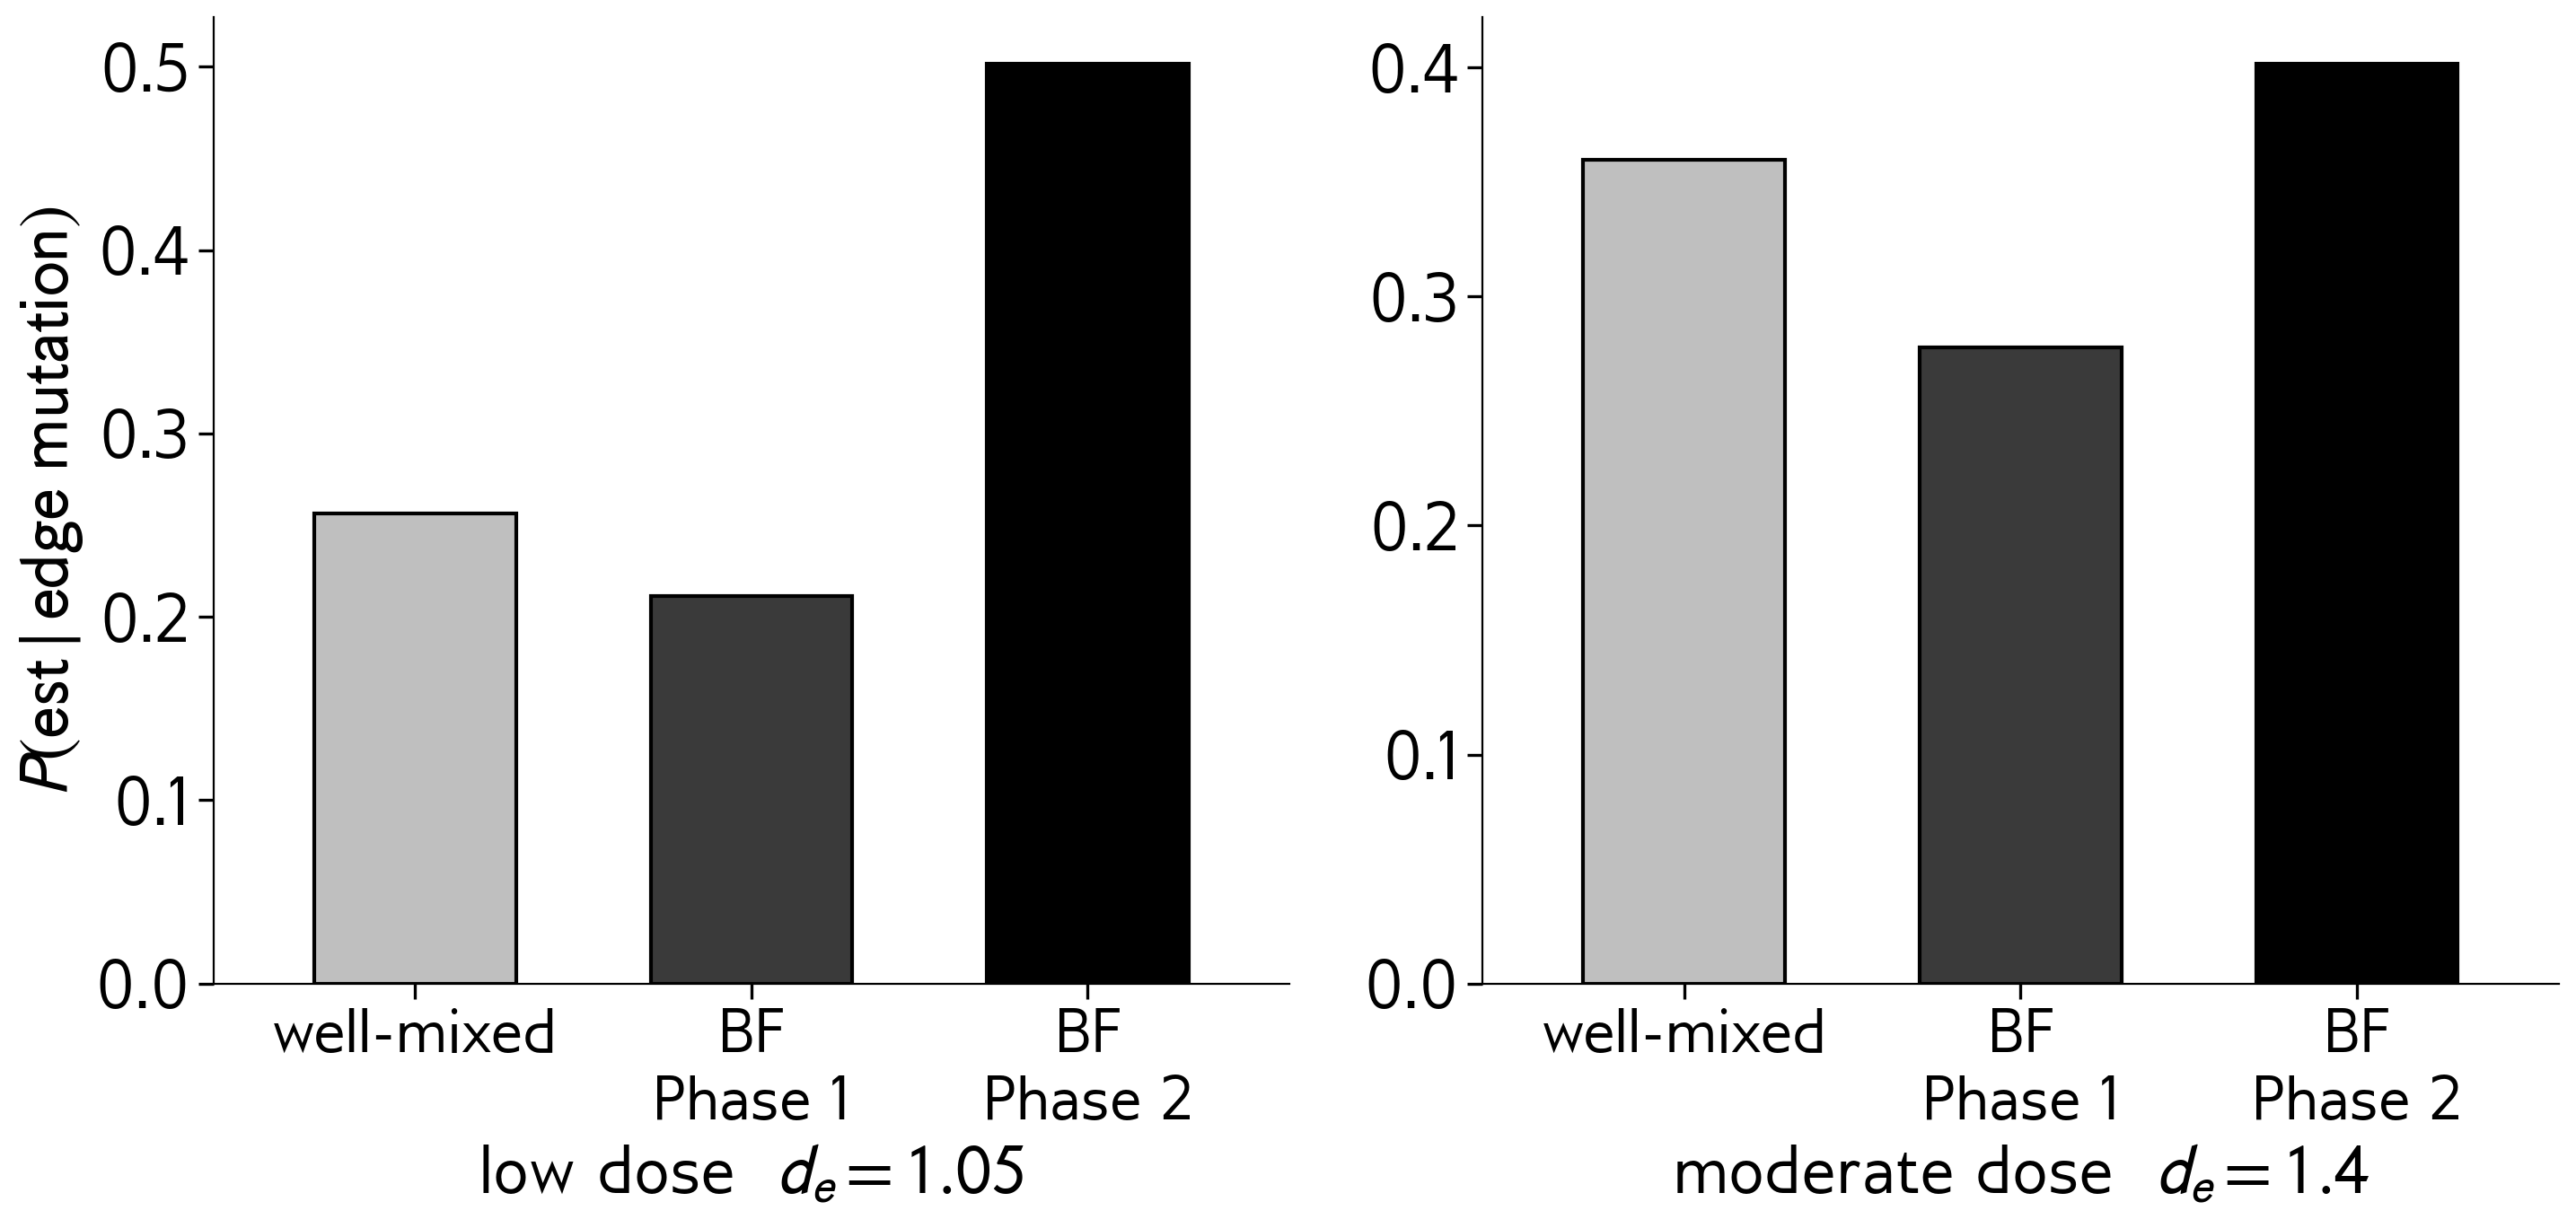
\includegraphics[width=0.92\textwidth]{estab_phase_bars.png}
\caption{Same comparison as Figure~\ref{fig:phaselines}, at a low dose
(left) and a moderate dose (right). Biofilm Phase 1 sits below
well-mixed; biofilm Phase 2 sits above. The contrast holds across
doses.}
\label{fig:phasebars}
\end{figure}

\paragraph{What it explains.} This mechanism settles the first of the
two questions from \S\ref{sec:doubleedge}. The biofilm always loses at
low dose because the buffered decline lasts a long time at low dose
(roughly $(N_0 - l)/(s_e l)$ in time units), so most edge-born
mutations are born during Phase 1, where they are suppressed. There is
no escape from this regardless of core activity: WT resupply is driven
by edge deaths pulling from the core, not by core births, so a dormant
core still resupplies. That is why the dormant biofilm in
Figure~\ref{fig:doubleedge} loses too. It is also why the per-mutation
establishment fraction in Figure~\ref{fig:decomposition}B is uniformly
lower for the biofilm than the well-mixed reference: most mutations
land in Phase 1, where the suppression is in effect.

What this mechanism does \emph{not} explain is why the biofilm with an
active core ever wins. The per-mutation tax operates whether the core
is active or dormant, so suppression alone would predict that an active
biofilm should lose, just by a different margin. The second track---why
an active core produces so many extra mutations, and what those
mutations do at high dose---is the subject of the next section.
\fi

\end{document}
